\chapter{Introducci'on}
% 
% Existen dos tipos de citas bibliograf'icas: usa \verb|\citep{..}| para
% citas en \emph{par'entesis} y \verb|\citet{..}| para citas
% en el \emph{texto}. Por ejemplo, estudios reciente han mostrado nuevos e
% interesantes modelos que se pueden aplicar para reformular teor'ias
% f'isicas~\citep{NewCam97}. Mientras que, el trabajo de \citet{Rofl06} fue
% considerado muy divertido por una significativa fracci'on de la comunidad
% de investigadores. Tambi'en es posible citar a varios trabajos en una sola
% referencia \citep{Lamport86,Knuth84}.



\section{Estructura de este trabajo}

Este primer capítulo introductorio está dividido en dos secciones que presentan los aspectos necesarios para comprender el trabajo realizado, el cual se centra en el diseño de nuevas secuencias linkers con 
propiedades conformacionales definidas, restringiendo cualquier actividad biologica y elemento estructural no deseado.
En la primer sección (\ref{proteinLandscape}) se intenta describir el amplio panorama conformacional y funcional que pueden presentar las proteinas, 
identificando cuales son los elementos funcionales que pueden de acuerdo a las propiedades estructurales que adquieren.
% in-vivo, describiendo cuales son los posibles destinos de las proteinas desde que son sintetizadas en el ribosoma y a lo largo de su etapa funcional en la célula. 
% Se desarrollan los conocimientos actuales acerce del perfil de conformaciones y funciones conocidas, y las propiedades secuenciales asociadas con estas.
% Se intenta describir como estos conocimientos actuales sobre las propiedades conformacionales y funcionales de las proteinas se trasladan en el desarrollo 
% de un amplio abanico de metodos y herramientas bioinformaticas que, a su vez, permiten nuevos avances en los conocimientos subyacentes.
En la sección siguiente (\ref{proteinEngineering}) se desarrolla el tema de ingenieria de proteínas, intentando mostrar los conceptos mas relevantes del área asociados a este trabajo, 
introduciendo el problema de diseñar nuevas secuencias linker.

En el capítulo \ref{method} se detalla el método implementado para obtener secuencias linker, indicando los fundamentos, limitaciones y aspectos relevantes de su utilización.

En el capítulo \ref{tools} se detalla el conjunto de herramientas utilizadas para evaluar propiedades estructurales y funcionales de interés, describiendo el objetivo de cada evaluación y los fundamentos de cada método. 

En el capítulo \ref{manual} se documentan todos los aspectos necesarios para poder obtener y hacer uso de la herramienta.

En el capítulo \ref{results} se muestran, en primer lugar, las evaluaciones realizadas para obtener los parámetros óptimos de ejecución. 
Además, se evalúan distintas propiedades de la herramienta resultante y su ejecución analizando, luego, las secuencias obtenidas. 

Finalmente, el capítulo \ref{conclusiones} contiene las discusiones relevantes, conclusiones y trabajo a futuro.































\section{Perfil conformacional y funcional de proteinas}\label{proteinLandscape}

% HAGO UNA INTRODUCCION A TODO EL TEMA DE CONFORMACION-FUNCION-HOMEOSTASIS-ETC, Y VOY REFERENCIANDO LAS DISTINTAS SUBSECCIONES
% PRIMERO HABLO DE LA RELACION UNA SECUENCIA-UNA ESTRUCTURA

Las primeras proteínas estudiadas poseían una tendencia intrínseca a plegarse espontáneamente para dar una única estructura tridimensional.
Los primeros estudios estructurales sobre estas proteinas indicaban que la información requerida para adoptar esta estructura estaba codificada en su secuencia primaria y que, además, se correspondia con un mínimo global sobre el
perfil de energía libre asociado al polipéptido.  
% Much research has been carried out since then into the mechanism of folding, both under carefully controlled conditions in the laboratory and within cellular environments

Es decir, la secuencia de AAs determina una unica estructura resultante, conocida como estructura nativa, la cual debía conferirle la función propia a la proteína.
Comenzaron a surgir, entonces, distintos modelos para explicar como 
Por un tiempo todo pareció indicar(y la mayoría acordó pensar) que una estructura plegada, aunque dinámica, era la base del mecanismo funcional en las proteínas.

% ACA PASO A LA IDEA DE POSIBLES DIFERENCIAS CON ESTE PARADIGMA CLASICO
El paradigma cambió rotundamente cuando se encontró que, a pesar de no poseer una estructura plegada claramente determinada, una gran cantidad de péptidos y proteínas poseía funciones biológicas relevantes,
principalmente cumpliendo roles de señalizacion y regulación, siendo capaces de interactuar con diversos elementos a través de distintos mecanismos.
Los siguientes estudios afirmaron que, efectivamente, estos elementos pueblan un ensamble de conformaciones considerablemente distintas, que varían en el tiempo, entre las distintas regiones de una misma secuencia y dependiendo del contexto.
La definición de estado nativo, cuyo criterio es identificar la capacidad de realizar una función biológica, debe aplicarse tambien sobre esta diversidad de conformaciones.



El estudio de los perfiles de energía libre también se ve modificado. 
Además, independientemente de su naturaleza estructural, se encontró que el estado nativo representa, probablemente, sólo un mínimo local bajo condiciones fisiológicas.
Esto se debe a que los estados de agregación representan generalmente, estados termodinámicamente muy estables correspondientes minimos globales. 
A partir de esto surgen nuevas preguntas acerca de cómo se mantiene en la célula la solubilidad de los estados nativos.
La respuesta entra dentro de un concepto más amplio conocido como proteostasis(u homeostasis de las proteínas), que se desarrolla hacia el final de esta sección.

% Wright and Dyson 8 suggested that the existence of proteins with intrinsic protein disorder calls for a reassessment of the protein–structure– function paradigm.
Con el tiempo, entonces, se fue encontrando que las proteínas podían tomar caminos distintos al plegamiento espontáneo y llegan a poblar diversos estados bajo condiciones fisiológicas, 
entre los cuales se encuentra un amplio rango de conformaciones desordenadas y parcialmente plegadas, e incluso distintos estados de agregación con características estructurales diversas.
La idea central de esta sección es mostrar como las proteinas pueden, entonces, pueden caer en un continuo de conformaciones estructurales y cómo las funciones 
emergen a partir de los distintos estados conformacionales y las transiciones dinamicas entre éstos.
% from tightly folded single domains, to multidomain proteins that might have flexible or disordered regions, to compact but disordered MOLTEN GLOBULES and, finally, to highly extended, heterogeneous unstructured states.

Los elementos estructurales y funcionales(y las relaciones entre estos) que permiten formar el paisaje resultante de conformaciones y actividades biológicas, 
se muestran en la última sección como modulos individuales que proveen a la evolución la capacidad de crear nuevas proteínas compuestas, dando un punto de vista mas arquitectónico de éstas.
% que pueden componerse para dar origen a proteinas con funcionalidades compuestas.
% Algunos de estos módulos le brindan a la naturaleza la dinámica evolutiva necesaria para adaptar ciertas propiedades, mientras que otros permiten 
% proveen un completo set de elementos y mecanismos funcionales a la célula. 




































\subsection{Conformación de proteínas en solución} \label{conformationalLandscape}

% \subsubsection{Proteinas globulares, fibrosas y de membrana}

% FALTA TODO LOS DE ESTRUCTURAS PLEGADAS

% ACA EMPIEZO A HABLAR DE FLUCTUACIONES EN LA CONFORMACION, Y QUE NO SON TOTALMENTE ESTÁTICAS

El paradigma clásico de la biología estructural afirma que la secuencia primaria de una proteína contiene la codificación para que esta adopte una 
Si bien esta idea es una simplificación, dado que aún las proteínas mas estables son sistemas dinámicos que poseen distintos grados de flexiblidad, este modelo se adapta a una gran cantidad de proteínas.
En éstas, el ensamble conformado por los estados accesibles en condiciones fisiológicas está conformado por un conjunto de estructuras que solo difieren en leves desviaciones del promedio del ensamble.
La dinámica de estas estructuras está dada por movimientos que varían entre fluctuaciones rápidas de pequeña amplitud(del orden de \AA) hasta cambios relativamente lentos($\mu$s - $s$) que involucran cambios estructurales relevantes(plegamiento y movimientos asociados a la función)
Todos los movimientos son resultantes de rupturas y formaciones de interacciones provocadas por fuerzas de interacción las cuales, debido a su naturaleza débil pueden romperse por efecto de la energía térmica, aún a temperatura ambiente.
Por lo tanto, a pesar de que estas proteínas puedan ser asociadas con estructuras estáticas definidas, las mínimas fluctuaciones térmicas de la temperatura ambiente les permite explorar distintas conformaciones como parte de su actividad biológica.
En general, todos estos movimientos están asociados al mecanismos por el cual ejercen su función.
El conjunto de proteínas que posee estas características estructurales son las que denominamos plegadas y, debido a estas mismas propiedades de poseer ensambles conformacionales con poca variabilidad, sus estructuras fueron las primeras que pudieron ser resueltas con precisión. 


% No se puede pensar, sin embargo, que todas las proteínas tendrán esta conformación plegada.
% Incluso entre las estructuras almacenadas en la PDB, no todas proteínas muestran una conformación definida a lo largo de toda su secuencia.
Es así que muchas de estas proteínas contienen segmentos no determinados de sus estructuras, 
usualmente esta falta de información es producto de regiones no definidas en el mapa de densidad electrónica que resulta del análisis de difracción por rayos X, 
correspondientes a ensambles de estructuras muy variables asociados a conformaciones flexibles o desordenadas. 
% Este tipo de segmentos es bastante común ya que sólo una pequeña porción de las estructuras en la PDB se encuentra totalmente libe de regiones con densidad electrónica no definida.
La simple pregunta sobre cuál es la conformación real que adoptan estos segmentos donde se pierde la definición en la densidad electrónica, junto con la aparición de diversas proteínas funcionales sin una estructura definida, 
llevaron a centrar la atención en aspectos de flexibilidad estructural y, particularmente, en los detalles de conformación de proteínas que no se adaptan correctamente al modelo clásico de plegamiento.
% further opened eyes toward flexibility and focused attention on proteins basically distinct from well-known globular proteins. 
% En terminos biofísicos, estas y otras questions such as, “what does the missing electron density in most of the deposited structures in the PDB correspond to?”, 
La búsqueda de respuestas a estos nuevos problemas llevo a descubir toda un area quizás más compleja (e incluso más amplia) que la determinada por el paradigma clásico de proteínas plegadas.

% “why are some proteins highly sensitive in vitro to proteolysis?”, and “why do some proteins possess a particular behavior during the purification process?” 






% ******************************************
% IDPs SECTION
% ******************************************

% La idea inicial de proteinas que adoptaban una estructura rigida pero levemente flexible parecía muy firme en un principio, principalmente por una gran cantidad de evidencias soportando la perdida de
% La idea de que las proteínas puedan adoptar estructuras 'desordenadas' era inaceptable inicialmente, 
% principalmente por la gran cantidad de evidencia sobre los requerimientos de 
Inicialmente, gran cantidad de evidencia soportaba la idea que la funcionalidad de las proteínas estaba asociada a su estructura tridimensional bien definida pero dinámica.
Consecuentemente, la idea de que muchas proteínas o regiones no adopten una estructura definida y posean una conformación intrínsecamente desordenada se creyo inaceptable. 
% Consequently, the notion that many proteins or regions of proteins could be not ordered, but were intrinsically disordered, was unacceptable for a long time.
Por lo tanto, durante un largo tiempo fueron identificandose y estudiándose experimentalmente una a una, tratándolas como excepciones al modelo clásico.
% These proteins were independently discovered one-by-one over a long period of time and therefore they were considered as rare exceptions to the general rule.
Luego de este proceso, hace al menos una década se formalizó la idea que el estado adoptado en condiciones nativas(funcionales) de muchas regiones o proteínas enteras podía ser intrínsecamente desordenado
(a partir de ahora intrinsically disordered region/protein = IDR/IDP).
% Only around the turn of the millennium was it eventually formally raised in several conceptual papers [1–3], among them one in TiBS [4], that many proteins or regions of proteins 
% are intrinsically disordered (IDPs, or as originally termed, unstructured) under native, functional conditions. Although it was based on rather limited evidence, the groundwork of
% the new field was laid and sparked an immediate rapid expansion.
% Varios reviews en \cite{uversky2010understanding,dyson2005intrinsically}.
Es decir, existe un conjunto cada vez mas amplio de proteinas cuya secuencia codifica conformaciones intrinsecamente desordenadas sin un plegamiento determinado.
% Estamos hablando de un numero considerable de proteinas cuya secuencia encodes for the intrinsically unstructured proteins without specific structure.
These raise several compelling biophysical questions related to the structural characteristics of natively unfolded proteins. 
How unfolded are these proteins? Are they random coils, or do they possess residual structure? If they have residual structure, how should they be classified?
% Based on the analysis of the available literature, it has been concluded that intrinsically unstructured proteins do not possess uniform structural properties, as expected for members of a single thermodynamic entity.
Un mayor avance en este nuevo campo ocurrió porque estas propiedades podían ser estudiadas utilizando una gran cantidad de técnicas biofísicas \cite{eliezer2009biophysical}.

% Structural disorder can now be studied in great detail by several dozen experimental techniques 
% and the most spectacular advance has been achieved through the application of multidimensional NMR. This approach is often
% complemented by other structural techniques, such as small-angle X-ray scattering (SAXS), which is combined with advanced computational data integration based upon molecular dynamics (MD) simulations (Figure 1). These new
% approaches [22] enabled the characterization of the full structural ensemble of several dozen IDPs
% 

% CONCEPTOS GENERALES !!! REESCRIBIR-REORDENAR
En general, las IDPs no poseen un centro hidrofóbico como para plegarse espontáneamente, lo que si ocurre en proteínas plegadas(en algo similar a un colapso hidrofóbico).  
% In general, proteins with intrinsically disordered sequences cannot bury sufficient hydrophobic core to fold spontaneously into the highly organized 3D structures that characterize the proteins that are represented in the Protein Data Bank.
En algunos casos, sin embargo, pueden formar estructuras desordenadas pero compactas, o algunos segmentos de la secuencia pueden adoptar transitivamente estructuras secundarias individuales.
% In some cases, compact but disordered molten-globule-like states can be formed, or local regions of the sequence can have a propensity to adopt isolated and fluctuating elements of secondary structure 
% (which is equivalent to the ‘pre-molten globule’ proposed by Uversky 2 ). 

% Due to their heteropolymeric nature, proteins are never random coils and always have some residual structure.
A pesar de esta tendencia desestructurada, debido a la naturaleza heteropolimérica de las proteínas, es probable que nunca adopten 
conformaciones totalmente aleatorias(where only local steric interactions constrain the conformations adopted by the molecule), incluso en entornos altamente desnaturalizantes.
Es decir, incluso los estados mas desestructurados mantienen una cierta tendencia a formar elementos estructurados locales, caracterizados por estructuras secundarias o núcleos hidrofóbicos.
La existencia de estos residuos de estructura se han detectado en proteinas estructuradas sometidas a altas concentraciones de desnaturalizantes fuertes. 
% Due to the heteropolymeric nature, it is probable that proteins rarely, if ever, behave as true random coils, especially in non-denaturing media: 
% even in their most highly unfolded states, proteins show a propensity to form local elements of secondary structure or hydrophobic clusters
% In fact, the existence of significant residual structure in the unfolded globular protein has been described even under the most severe denaturing conditions, such as high concentrations of strong denaturants [144-147]. 
% Accumulated data nonambiguously show that they most likely represent the polymer coils below a critical point, even under harsh denaturing conditions.
% Thus, coil-like ID proteins are not completely random, but are characterized by the presence of some residual (and highly flexible) structure. 

% Protein random coils differ from true random coils in important respects, such as a non-random population of internal bond angles along the chain.
% Thus, based on the exceptional structural heterogeneity of IDPs/IDPRs, IDPs are definitely much more structurally complex than random coil-like polypeptides.
Como vamos a ver, esta leve estructura residual(latente o transitiva) es muy importante para y representan gran parte de las capacidades funcionales en IDRs/IDPs.
% ....This fact is very important for the functioning of these proteins.
Por lo tanto, se puede decir que las IDRs/IDPs poseen propiedades conformacionales mucho mas complejos que polipéptidos con estructuras totalmente aleatorias y que esta excepcional heterogeneidad estructural
representa tambien un problema crítico a la hora de estudiarlas experimentalmente y caracterizarlas.
% Although this structural heterogeneity is very important for protein functionality, it represents a crucial hurdle for structural characterization of IDPs

% Coincidiendo con esta idea que la proteina no plegada nunca es una true random-coil, the persistence of native-like contacts in the denatured (disordered) state has been shown in NMR experiements and in high temperature molecular dynamics simulation. 
% The existence of preferred limited proteolysis cutting sites also indicates that the native conformation prevails

A partir de esta descripcion estructural se puede entender por que el termino inicial asignado a estas proteínas (proteínas desestructuradas) ha quedado obsoleto.
% These and many other studies made the term unstructured obsolete. 
La única característica distintiva de las IDRs/IDPs es, entonces, su inhabilidad para plegarse en una estructura tridimensional única.
% The distinguishing and unifying feature of these proteins,if any, is their inability to fold into a unique and stable tertiary structure.
A pesar de esta falta de estructura única definida, como se vió, presentan una gran diversidad de propiedades estructurales y, lo que es mas importante, estas están relacionadas con sus funciones. 
Por lo tanto, el término general para describir estas proteínas es, simplemente, 'desordenadas'.
% They display a vast array of function-related structural organization, therefore, the field has settled on the term ‘disordered’. 
Este término se aplica tanto a las regiones que forman parte de proteinas plegadas mas grandes, como a secuencias que carecen totalmente de estructura plegada. 
% This term applies to both short and long regions that are part of a larger folded protein (loops and linkers) and proteins that entirely lack a folded structure. 
% This latter category is sometimes also termed (natively) unfolded. 
Como veremos, el mosaico estructural que ofrece la variedad de secuencias con regiones de diversas propiedades estructurales es fundamental para obtener el extenso catálogo de funcionalidades existentes.    
% Como veremos..many proteins are hybrids of ordered and disordered domains and regions, and this mosaic structural organization is crucial for their functions.




% ******************************
% PROPIEDADES ESTRUCTURALES
% ******************************

Ahora que sabemos que no estan completamente libres de restricciones estructurales, nos concentraremos en cuales son esas propiedades conformacionales que si poseen....
Structurally, IDPs range from completely unstructured polypeptides (native coils, that resemble the highly unfolded states of globular proteins) 
to extended partially structured forms (native pre-molten globules) or even to compact disordered ensembles that may contain significant secondary structure (native molten globules)
% ID proteins have dynamic structures that interconvert on a number of timescales and have been shown to have many similarities to non-native states of “normal” globular proteins, 
% which(como se describio antes) may exist in at least four different conformations: native (ordered), molten globule, pre-molten globule, and coil-like.
Indeed, they consist of dynamic structures that interconvert on a number of time scales.
This distribution is constantly changing in time where a given segment of a protein molecule has different structures at different time points. 
As a result, at any given moment, an IDP has a structure which is different from a structure viewed at another moment


A pesar de esta dinámica estructural, by definition, IDPs are devoid of stable!!! secondary and/or tertiary structures under physiological conditions.
However, a majority of them have some residual transient secondary structures that are required for function.
A typical IDP/IDPR contains a multitude of elements coding for potentially foldable, partially foldable, differently foldable, or not foldable at all protein segments.
Hence, it should be borne in mind that most proteins are neither fully ordered nor fully disordered but contain ordered and disordered regions at different ratios.
Este perfil conformacional forma un continuo estructural que puede verse en \ref{conformationContinuum}.
Indeed, only about 32\% of the crystal structures of the PDB are completely devoid of disorder and the degree or the depth of disorder (as it is manifested by the absence of the electron density) varies widely, 
suggesting that the fully ordered protein depicted in \ref{conformationContinuum}(y que habiamos visto al principio) is apparently the exception rather than the rule.


\begin{figure}[htbp]
\centering
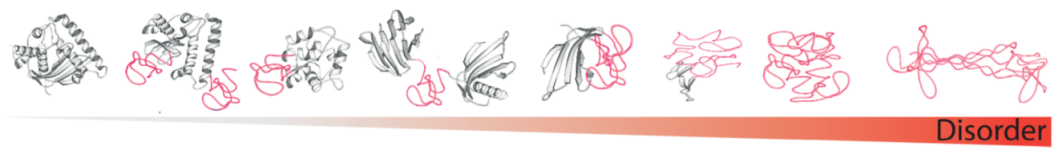
\includegraphics[width=1.0\textwidth]{img/conformationContinuum.png} 
\caption{Continuum of disorder. Functional disordered segments can be as small as only a few amino acid residues, or they can occupy rather long
regions or ends. Different levels of order and disorder. From left to right: no disorder; disordered N- and C-termini; disordered linker; disordered loop;
disordered domain; disordered protein with some residual structure; wholly disordered, mostly collapsed protein; wholly disordered, extended protein.
Corresponding disordered regions are shown in red.}
\label{conformationContinuum}
\end{figure}



% CLASIFICACION

However, already in some early studies, it was indicated that IDPs/IDRs could be crudely grouped into two major structural classes, proteins with compact and extended disorder, 
indicating that functional IDPs can be less or more compact and possess smaller or larger amount of flexible secondary/tertiary structure.

Para dejar las cosas un poco mas claras vamos a intentar realizar una clasificacion de las ID proteins en terminos estructurales.
Usando esta analogia(similitud) con los estados intermedios del plegamiento, en \cite{uversky2010understanding} it has been established that ID proteins and regions under physiological conditions in vitro might 
contain collapsed-disorder (i.e., where ID is present in a form of molten globules) and extended-disorder (i.e., regions where ID is present in a form of random coil or pre-molten globule)

\begin{itemize}
 \item Collapsed disorder:  The structural properties of the molten globule (which was originally described as universal folding intermediate of globular proteins) are well known and
have been systematized in number of reviews. The protein molecule in this intermediate state has no (or has only a trace of) rigid cooperatively melted tertiary structure. 
However, it is characterized not only by the well-developed secondary structure, but also by the presence of some topology, i.e., relatively fixed mutual positioning of the secondary structure elements.
A considerable increase in the accessibility of a protein molecule to proteases was noted as a specific property of the molten globule.
The transformation into this intermediate state is accompanied by a considerable increase in the affinity of a protein molecule to the hydrophobic fluorescence probes

 \item Extended disorder: A significant number of sequences encodes for the extendedly disordered proteins that are characterized by low sequence complexity. Are these proteins
random coils, or do they possess residual or transient structure? If they have residual or transient structure, how should they be classified? Based on the analysis of the available literature, it has been concluded that such proteins do not possess uniform structural properties, as expected for members of a single thermodynamic entity.
In fact, they may be divided into two structurally different groups, intrinsic coils and intrinsic pre-molten globules, tal como se realiza en \cite{uversky2002natively}: 
 Proteins from the first group have hydrodynamic dimensions typical of considerably unfolded polypeptide chain in poor solvent (see below and fig. 1), and do not possess any (or almost any) ordered secondary structure. 
Proteins from the second group are more compact (see below and fig. 1), and exhibit some amount of residual secondary structure. However, they are still less dense than native globular or molten globule proteins
\end{itemize}





















% DIFERENCIAS EN EL PERFIL DE ENERGIA LIBRE
The difference between folded proteins and disordered proteins can be understood based on an analysis of their free energy landscapes \ref{idp-folded-EnergyLandscape}.
Folded proteins have a "funnel-shaped" global free energy minimum, where the lowest energy state corresponds to the 11native structure, and the width of the unique global energy minimum
determines the conformational entropy of the native state.
By contrast, disordered proteins have multiple local energy minima separated by small(low-energy) barriers, which can be described by relatively flat energy landscapes.
Transitions between the different local energy minima occur quickly and often, leading to an ensemble consisting of a vast number of structurally dissimilar states, which have approximately equal energies. 
Thus, a comprehensive characterization of an IDP consists of an ensemble of states and the transition rates between them.

In practice, knowledge of the transition rates between conformers in an IDP ensemble is very difficult to capture, both experimentally and computationally. 
Consequently, in practice, studies of IDPs have focused on modeling the thermodynamically accessible states alone. As we outline below, while this represents an incomplete picture of these
proteins, a great deal of information and insight has arisen from such studies.


Estas secuencias presentan en solución un conjunto heterogéneo de conformaciones fácilmente maleable por cambios en el medio. 
Conditions, post-translational modifications, and binding events change the relative free energies of individual conformations as well as the energy differences between conformations.
As a result, the populations of individual conformations within the ensemble change under different conditions. 
These individual states are often important for function. Thus, the dynamic nature of IDPs is best modeled by statistical approaches that describe the
probabilities of individual conformations in the ensemble, and is best measured by experimental techniques that prevent conformational averaging.

En lugar del análisis estructural clásico basado en dominios globulares, podemos describir estos conjuntos conformacionales en términos de los promedios y desviaciones estándar de la distancia entre los extremos de la secuencia, el radio hidrodinámico, el contenido en estructura secundaria y otros parámetros (20).


\begin{figure}[h]
\centering
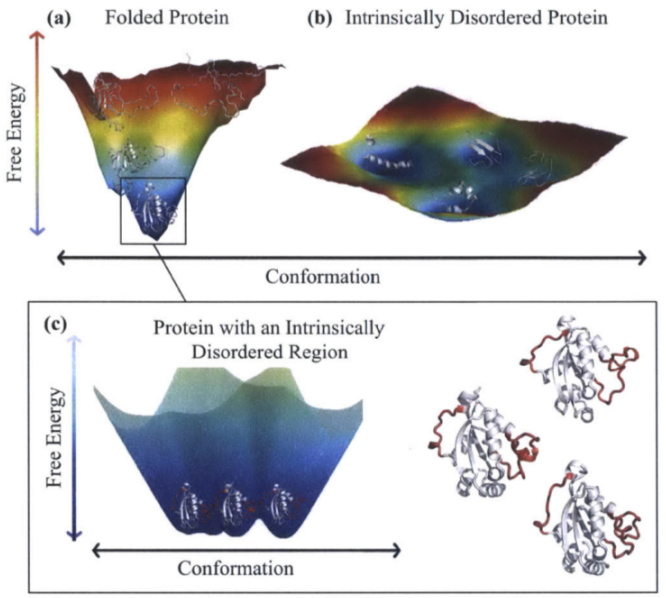
\includegraphics[width=0.7\textwidth]{img/idp-folded-EnLandscape.png} 
\caption{Diferencias en el paisaje energético entre polipéptidos que adquiren estructuras plegadas, IDRs e IDPs }
\label{idp-folded-EnergyLandscape}
\end{figure}







% ***************
%  INDUCED FIT:
% *****************
Although disordered proteins exist as dynamic structural ensembles without fixed(estable!!!) tertiary structures, there is evidence that many flexible regions of proteins undergo coupled binding and folding \cite{dyson2005intrinsically}. 
A large decrease in conformation entropy accompanies such disorder-to-order transitions. 
An important feature of the intrinsically unstructured proteins is that they are able to undergo a disorder-to-or-der transition (i. e. partial or complete folding) during or prior to their biological function. 
In other words, intrinsically unfolded proteins in vivo are likely to be stabilized by functional binding to specific targets and ligands (such as a variety of small molecules, substrates, cofactors, other proteins, nucleic acids, membranes and so on). 
% Many intrinsically disordered proteins undergo transitions to more ordered states or fold into stable secondary or tertiary structures on binding to their targets — that is, they undergo coupled folding and binding processes.

Functional complexes of IDPs with their partners are formed via the specific intermolecular interactions that change the energy landscape creating more defined free energy minima.
Esta diferencia se ve en \ref{idpBindingEnLandscape}


\begin{figure}[h]
\centering
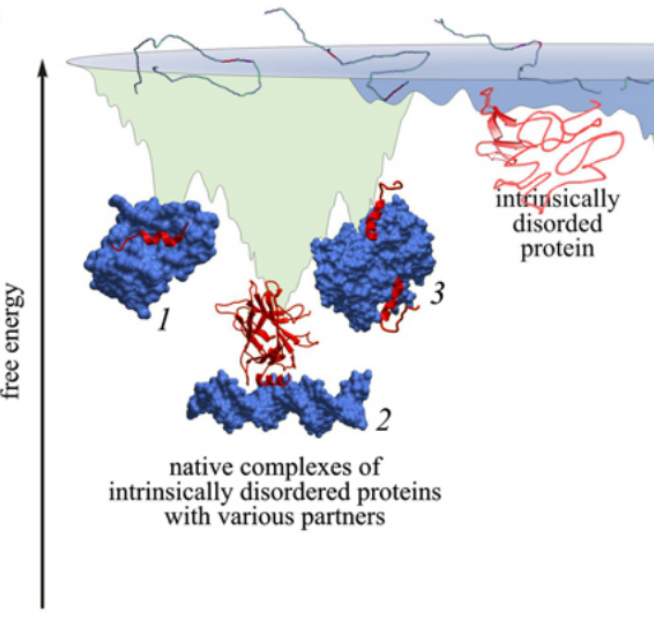
\includegraphics[width=0.7\textwidth]{img/idp-binding-EnLandscape.png} 
\caption{Perfil energetico de los estados de un polipeptido con estructura nativa desordenada. 
Disordered segments of these proteins can gain ordered structure at the interaction with specific binding partners in a case if the free energy of such complexes is lower 
than the free energies of the intrinsically disordered protein and its partner. 
1, 2, and 3 represents native complexes of intrinsically disordered proteins with various partners.
Por si solo, el polipeptido presenta a relatively flat energy landscape(sección derecha). Figura extraida de \cite{turoverov2010protein}}
\label{idpBindingEnLandscape}
\end{figure}


IDPs fold as a whole while interacting with their partners, if the free energy of complex is lower than the free energies of IDP and its partner before their interaction.
More often, however, only a part of an IDP, a specific recognition element, which is a relatively short amphipathic linear motif contained within long disordered sequence, is involved in the coupled folding and binding events
Induced fit interactions can also occur between structural domains and relatively large natively unstructured regions of other proteins. 
The natively unstructured region is then induced to form a stable structure, but only in the presence of the interacting structural domain.

This disorder-to-order transitions, in turn, leads to a combination of high specificity and weak affinity, a pair of linked features that are extremely useful for signalling and regulation.

An often-raised issue with respect to IDP binding is whether folding occurs before or after binding (termed conformational selection and induced folding, respectively).
Detailed studies suggest that folding can occur both before and after binding in distinct cases


There are two major models describing the coupled folding and binding process in proteins, the conformational selection model and the simultaneous binding and folding model, also known as the induced folding model.

The conformational selection mechanism is based on the hypothesis that when free in solution, IDP populates the ensemble of conformations and, from this ensemble, the binding partner “chooses” or
“selects” a specific conformation which closely approximates that of the bound form. An illustrative example of the conformational selection mechanism in the recognition process is
so-called “preformed structural elements” or elements of local residual structure, which are frequently observed in IDPs and which are crucial for the IDP interactions with its specific
partners

Induced folding model postulates that IDP associates with its binding partner in a fully disordered state and subsequently folds in association with the target protein. 
In molecular recognition, this model is exemplified by so-called molecular recognition elements or features, which are short (around 20 residues) structural elements which are found 
within the regions of disorder and which mediates certain classes of binding
events of disordered regions undergoing a disorder-to-order transition into a specific structure that is stabilized by binding to its partner.
These recognition motifs can fold into $\alpha$-helix, $\beta$-strand, or form irregular structure on binding to a target protein

Obviously, in reality, either one of the outlined above mechanisms, the conformational selection model or the induced folding model, or some combination of the two can be used.
Esto se ve representado en la figura \ref{idpBinding}



\begin{figure}[h]
\centering
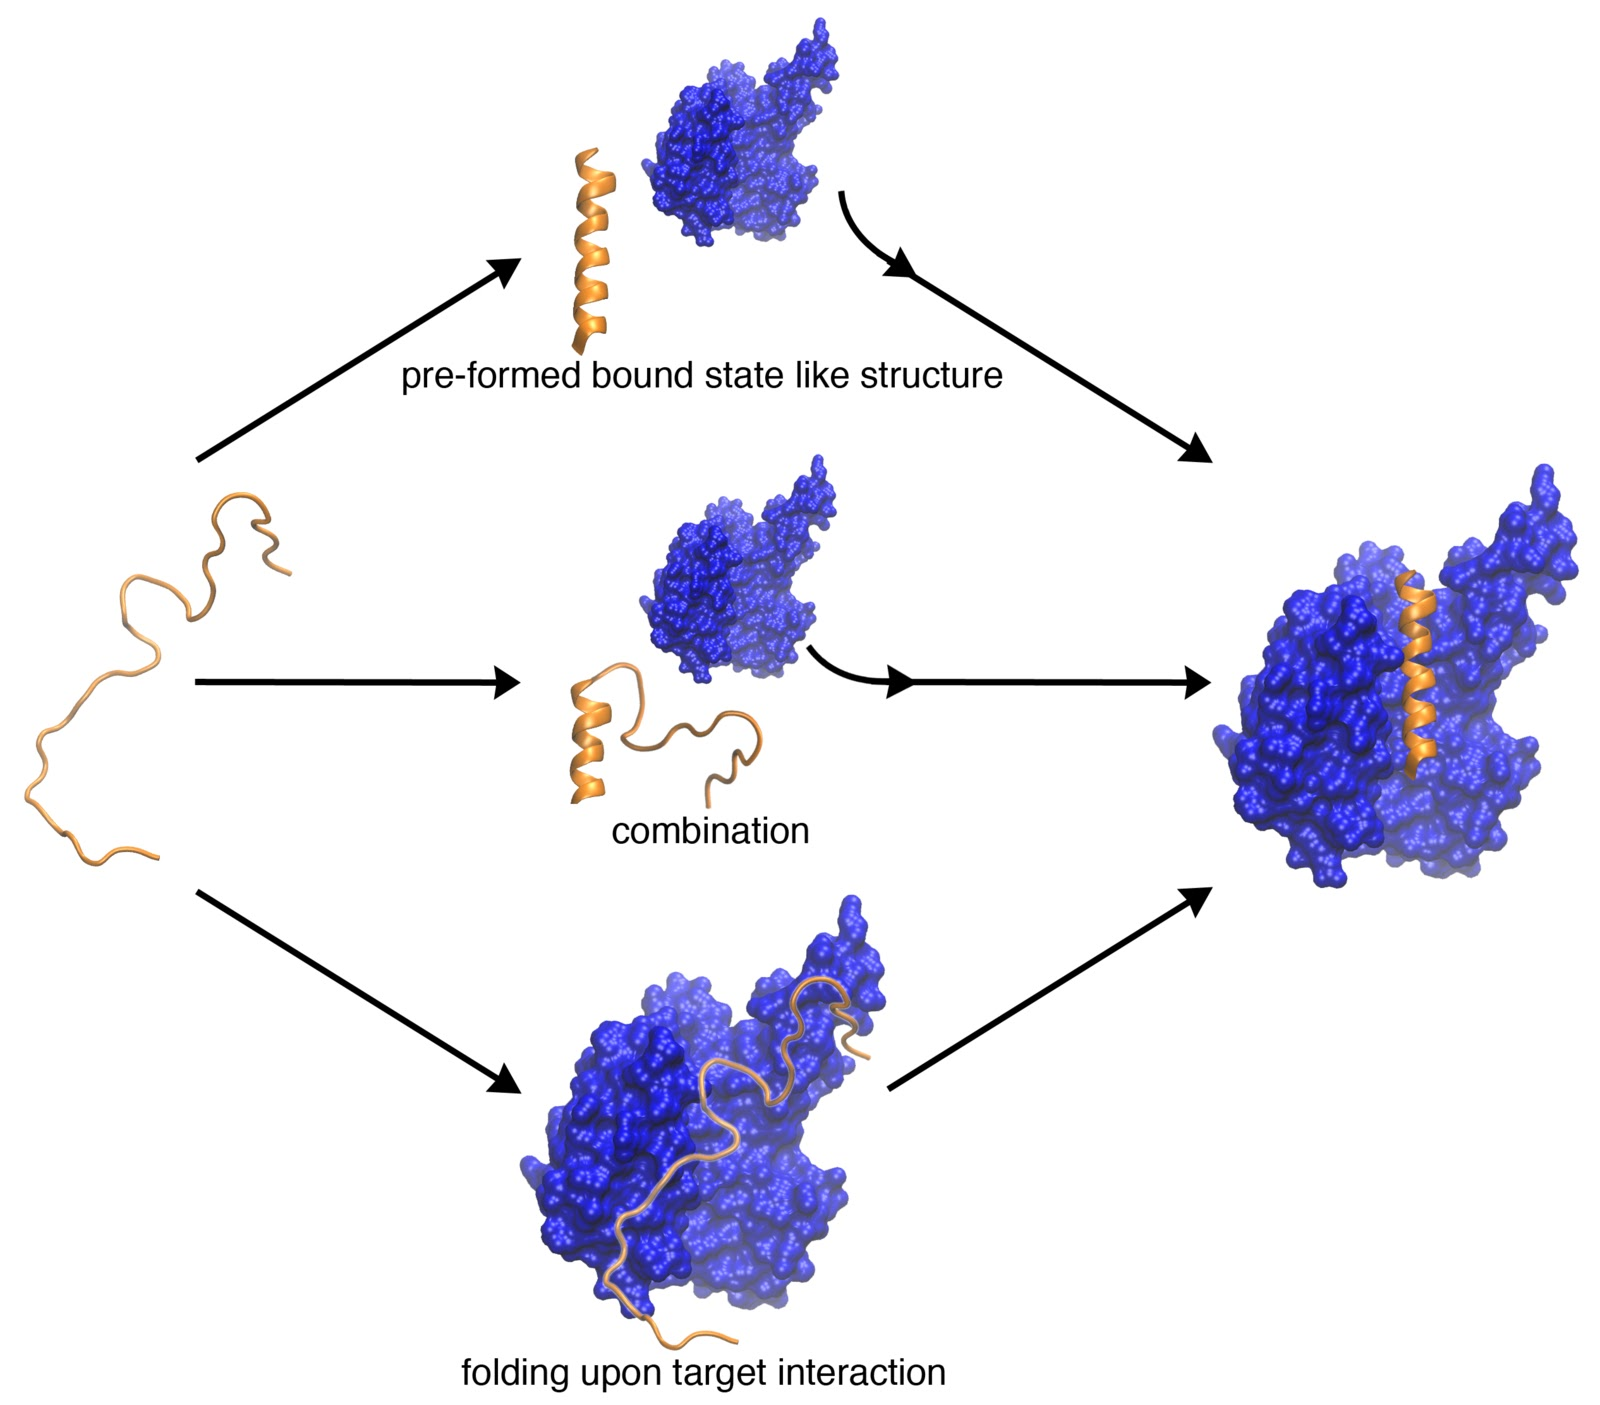
\includegraphics[width=\textwidth]{img/PSE-MoRE.jpg} 
\caption{Distintos modelos de binding para IDRs/IDPs} 
\label{idpBinding}
\end{figure}



% ESTO TIENE QUE IR DESPUES DE TODO EL DESARROLLO DE INDUCED FIT
En base a estas propiedades estructurales y el induced fit, en el review \cite{dunker2001intrinsically} se plantea una clasificacion del desorden en dos categorias: intermittent and constant.
The former describes protein molecular recognition domains and other regions that undergo order/disorder transitions to carry out binding or other functions. The latter describes regions such as
proteinaceous detergents, flexible linkers, entropic springs, entropic clocks and entropic bristles that remain disordered while carrying out function.

Two unexpected and important concepts have also emerged in the binding-folding paradigm. One is the intriguing observation that two IDPs/IDRs can bind each other in a process of mutual (synergistic) folding [47].
The other, even more confounding finding, is that recognition can proceed even in the lack of folding in the bound state. 
The many examples of such ‘fuzzy’ interactions demand the extension of the concept of structural disorder to the bound state.













% COMPOSICION CARACTERISTICA DE IDPs
Identification of IDPs as unique entities belonging to a new protein tribe is directly related to the recognition that their amino acid sequences are dramatically different from those of ordered proteins.
En otras palabras, since amino acid sequence determines three-dimensional structure, amino acid sequence should also determine lack of three-dimensional structure.

the absence of regular structure in these proteins has been explained by the specific features of their amino acid sequences including the presence of numerous uncompensated charged groups (often negative); 
 i.e., a high net charge at neutral pH, arising from the extreme pI values in such proteins , and a low content of hydrophobic amino acid residues.
Several ID proteins have been discovered due their unusual amino acid sequence compositions

It has been concluded that the combination of low mean hydrophobicity and relatively high net charge represents an important prerequisite for the absence of compact structure in proteins under physiological conditions.
% This observation was used to develop a charge-hydropathy (CH) plot method of analysis that distinguishes ordered and disordered proteins based only on their net charges and hydropathies.
From the physical viewpoint, such a combination of low hydrophobicity with high net charge as a prerequisite for intrinsic unfoldedness makes perfect sense: high net charge leads to charge-
charge repulsion, and low hydrophobicity means less driving force for protein compaction. In other words, these features are characteristic for ID proteins with the coil-like (or close to coil-
like) structures.
The disordered proteins are significantly depleted in bulky hydrophobic (Ile, Leu, and Val) and aromatic amino acid residues (Trp, Tyr, and Phe), which would normally form the hydrophobic core of a folded globular protein, and also possess low content of Cys and Asn residues.
The depletion of ID protein in Cys is also crucial as this amino acid residue is known to have a significant contribution to the protein conformation stability via the disulfide bond formation or being involved in coordination of different prosthetic groups.
On the other hand, ID proteins were shown to be substantially enriched in polar, disorder-promoting, amino acids: Ala, Arg, Gly, Gln, Ser, Glu, and Lys and also in the hydrophobic, but structure braking Pro.

% The fact that natively unfolded proteins, with their depleted hydrophobicity, are noncompact under physiological conditions indicates that ‘salted water’ (typical ‘physiological’ buffer contains 100–150 mM NaCl) does not represent for them a poor solvent.
% In other words, these conditions do not force polymer segments to interact specifically with each other and, thus, do not force them to be effectively excluded from the solvent.
% On the other hand, it has already been noted that even high concentrations of strong denaturants do not represent a good solvent for a polypeptide chain encoding for a typical globular protein, and a globular protein was assumed to never be a random coil.

En terminos biologicos, 
The fact that the sequences of ordered and disordered proteins and regions are noticeably different suggested that IDPs clearly constitute a separate entity inside the protein kingdom, 
that these proteins can be reliably predicted using various computational tools,  and structurally, that IDPs should be very different from ordered globular proteins since peculiarities of amino acid sequence determine protein structure.

% Por lo tanto, a signature of probable intrinsic disorder is the presence of low sequence complexity and amino-acid compositional bias, with a low content of bulky hydrophobic aminoacids (Val, Leu, Ile, Met, Phe, Trp and Tyr), which would
% normally form the core of a folded globular protein, and a high proportion of particular polar and charged amino.....
% ESTAS PROPIEDADES SE HAN UTILIZADO PARA LAS PRIMERAS GENERACIONES DE HERRAMIENTAS PARA PREDECIR DESORDEN A PARTIR DE LA SECUENCIA.
% Luego se crearon predictores que analizaban la secuencia usando ventanas(PONDR)

% In addition to amino-acid composition, the disordered segments have also been compared with the ordered ones by various attributes such as hydropathy, net charge, flexibility index, helix
% propensities, strand propensities, and compositions for groups of amino acids such as W + Y + F (aromaticity).

% Estas propiedades fisicoquimicas tambien fueron incluidas para los predictores.




% COMENTARIOS APARTE SOBRE LA REGULACION DE IDPs EN LA CELULA
It is clear now that the IDPs and IDPRs are real, abundant, diversified, and vital. The highly dynamic nature of IDPs and IDPRs is a visual illustration of the chaos.
the evolutionary persistence of these highly dynamic proteins (see below), their unique functionality, and involvement in all the major cellular processes evidence that this chaos is tightly controlled

Todas estas propiedades hacen que parezca razonable que este tipo de proteínas este altamente regulada dentro de la célula \cite{gsponer2008tight}.

Ademas por la extrema sensibilidad que tienen a la proteolisis in-vitro (lo cual es de esperar dada la confomracion extendida que adoptan), 
existen mecanismos para regular su degradacion(ver \cite{habchi2014introducing} Survival of IDPs in the Cell )





















































\subsection{Misfolding \& Aggregation}



% INTRODUCCION

En la seccion anterior vimos como algunas proteinas poseen conformaciones nativas con estructuras bien definidas.
Este restriccion hace que, para poder funcionar correctamente deban atravesar un proceso de plegamiento, el cual ocurre, normalmente muy rapidamente, dado que 
the sequences of these proteins have evolved in such a way that their unique native states can be found very efficiently even in the complex environment inside a living cell.
Sin embargo, as the size and complexity of proteins increase, therefore, the folding process becomes more complex,
thus, errors along folding may occur and drive proteins to incorrectly folded or misfolded states, which may still possess certain stability in the physiological
environment and, therefore, start to accumulate. 
Ademas....
Intermediates with only partially formed structures can be populated and have significant lifetimes. 
Under some conditions, then, proteins fail to fold properly or to remain correctly folded; this misfolding can lead to malfunction of proteins and the development of different pathological(cambio esta palabra??) conditions.
In addition, events that may be termed 'misfolding' may take place during the search for the stable native-like contacts between residues. 
That such complexities are seen even in the benign environment of a dilute solution of a pure protein suggests that they are even more likely to occur in the crowded environment of the cell.

Protein misfolding is a wide-spread phenomenon. Any protein with changes in native structure which affect its normal function is misfolded. 
The terms 'misfolded' and 'aggregated' are not equivalent. Como se verá, la habilidad de una proteina formar agregados desestructurados o fibras depende de muchos factores, including protein sequence and environment.
De otra forma, las proteinas que adquieran conformaciones no estructuradas o que se encuentren en estados de plegamiento intermedios semi-estables tendrían una gran tendencia a la agregación, sin embargo esto no es así. 
% De hecho, sólo una pequeña fraccion de tales conformaciones tiene tendencia a formar agregados.

% But the idea that proteins can misfold, or fold to intermediates that may undergo undesirable reactions such as aggregation, provides insight into potential problems that can arise during folding even in the best designed environments.
% Folding and unfolding are also now known to be coupled to many of the key events in the functioning of a biological system, including translocation of proteins across membranes, protein trafficking, 
% secretion of extracellular proteins, and the control and regulation of the cell cycle.
% Thus, the failure of proteins to fold or to remain folded under physiological conditions is likely to cause malfunctions and hence disease







% **************** AGGREGATION

The abnormal association of misfolded proteins usually leads to the formation of aggregates. 
Small aggregates can remain soluble, but large protein aggregates precipitate out of solution under physiological conditions. 
From the morphological point of view we can differentiate essentially two types of aggregates: amorphous aggregates and amyloid fibrils. 
Amorphous aggregates display a granular appearance when imaged by electron microscopy and consist mostly of disordered polypeptide chains, even if they
display certain regions enriched in $\beta$-sheet structures, which glue the macromolecular assembly.
Por otro lado.....Amyloid fibrils are highly ordered and repetitive structures where all polypeptides adopt a common fold.
Si bien no se van a dar detalles puntuales de la estructura, se sabe que estas diferencias que se ven en la estructura macromolecular son el reflejo de diferencias en las interacciones y estructura a nivel atómico.
These differences in structure also reflect biological differences; amyloid and amorphous beta-sheet aggregates have different chaperone affinities, accumulate in different cellular locations and are degraded by different mechanisms.
Contrary to amorphous aggregates, amyloid structures can fulfill biological functions, and functional amyloids are found in organisms from prokaryotes to humans \cite{fowler2007functional}.



% 
% Proteins might aggregate utilizing relatively short sequence stretches, usually organized in b-sheet-like assemblies. 

% La idea construida en las secciones previas, en la que un polipéptido nasciente podía adopar un continuo de conformaciones estructurales monoméricas y solo formar interacciones transitivas para cumplir si función, 
% debe extenderse ahora para incluir este conjunto de posibles estados de agregación. 
% En la sección previa se formó la idea que un polipéptido nasciente podía adoptar un continuo de formas conformacionales diferentes, con elementos diferentes

La idea construida en las secciones previas, en la que un polipéptido podía adopar un continuo de conformaciones estructurales monoméricas y formar interacciones transitivas con ligandos,
se le deben agregar ahora todos los posibles caminos alternativos que involucran formación de estructuras estables de agregación.
En la figura \ref{aggregationDiagram} pueden verse, de forma gráfica, distintos estados de agregacion como caminos alternativos al camino central de plegamiento/conformación monomérica.
% De la figura puede verse también, que los distintos procesos de agregación, que resultan en disintas estructuras agregadas, pueden originarse a partir de distintos estados iniciales de conformación.

\begin{figure}[h!,centered]
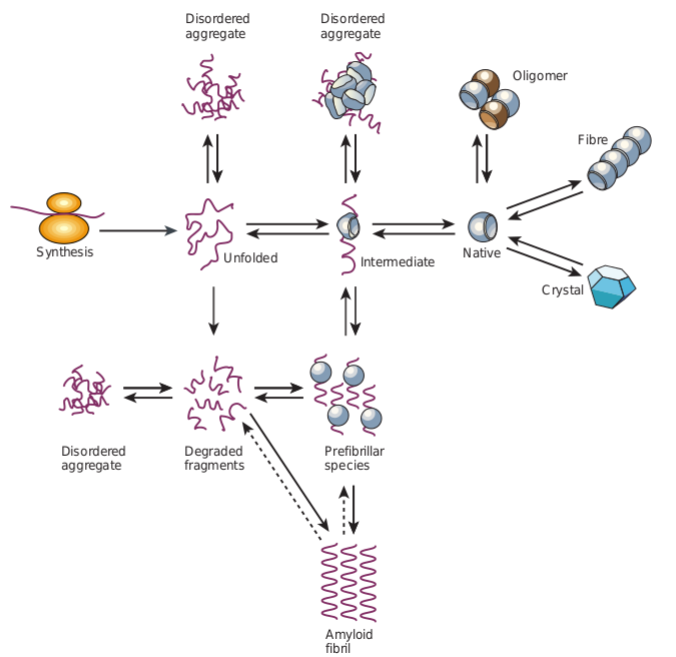
\includegraphics[width=\textwidth]{img/aggregationDiagram.png} 
\caption{Equilibrio de los estados de agregación} \label{aggregationDiagram}
\end{figure}


De la figura....
One should distinguish between precipitates, in which proteins maintain the native folded conformation and aggregates, in which proteins adopt new non-native structures. 
The first type of self-assembly is generated during random precipitation of already native protein due to an environment promoted reduction of solubility in the polypeptide chain. 
Examples of these processes are salting out by ammonium sulfate or isoelectric precipitation, que son los procesos utilizados para obtener los cristales que se utilizaran en la resolución de estructuras por difracción de rayos X. 
Reducing ionic force or shifting solution's pH results in immediate dissolution of these precipitates. 
The second type of macromolecular structures exhibits, without exception, an increase in $\beta$-sheet secondary structure content relative to the native conformation and
very high concentrations of denaturants or detergents are needed to dissolve them into mainly unfolded polypeptide chains. 
We will focus our attention on these aggregates, which include amyloid fibrils, thermal aggregates and bacterial IBs. 







% ***********************************************************
% *******          AMYLOIDS
% ***********************************************************

Lo que se ve al parecer en la figura \ref{aggregationDiagram} es que...
Amyloid are just one of the types of aggregate that
can be formed by proteins.
Sin embargo....
% ACA PONGO MUY EN GENERAL ALGUNAS PROPIEDADES DE LAS FIBRAS AMILOIDES COMO PARA EMPEZAR A HABLAR DE ESTO
Similar to globular native states, amyloid structures are closely packed and highly ordered
Although, a significant feature of this particular species is that its highly organized hydrogen-bonded structure is likely to give it unique kinetic stability. 
Thus, once formed, such aggregates can persist for long periods, allowing a progressive build-up of deposits in tissue, and indeed enabling seeding of the subsequent conversion of additional quantities of the same protein
into amyloid fibrils.




% CONCEPTOS GENERALES DE LA ESTRUCTURA
The amyloid state was first observed in the context of systemic amylodidosis more than 150 years ago, and indeed the name ‘amyloid’ means ‘starch-like’, 
as the deposits observed in the tissues and organs of patients who died from these conditions contained deposits that stained
with iodine, which is used to detect starch. Since then, it has been found that the proteinaceous deposits extracted from tissues in misfolding diseases
typically have amyloid characteristics. Such deposits are usually primarily composed of one protein, although they are typically associated in vivo with various other molecules.
% Remarkably, there is no evident similarity in the sequences, native structures or functions of the group of disease-associated proteins. 
% Despite such differences, the corresponding amyloid fibrils all contain a common cross-$\beta$ pattern in X-ray fibre diffraction studies that is indicative of the component $\beta$-strands being oriented
% perpendicularly to the fibril axis. Moreover,in solid-state magic angle spinning NMR spectroscopy studies, the typically high-resolution nature of the amyloid fibril spectra provides direct evidence for extensive regions of highly ordered molecular structures within the
% fibrillar environment

Amyloid aggregates are characterized by a particular fibrilar morphology 
% under transmission electron microscopy (TEM), 
which is highly ordered, compact, stable
and unbranched. This type of structures are denominated amyloid fibrils, their diameters range within tens of nanometers and their longitude can reach several
micrometers; mature fibrils can further associate laterally to form fibers.
All amyloid fibrils share the a common architecture composed of cross-$beta$ supersecondary structure,
where parallel $beta$ -sheets extend with their strands facing to each other and perpendicular to the fibril axis; 
such a conformation se encontro inicialmente ya que mostraban a characteristic X-ray diffraction pattern that is indicative of the component $\beta$-strands being oriented
perpendicularly to the fibril axis. 
The cross-$/beta$ architecture provides very great stability to the fibrils, as it allows the formation of a continuous array of hydrogen bonds

A diferencia de esta similitud en las estructuras encontradas...Amyloidogenic proteins are quite diverse, with little similarity in sequence and native three-dimensional structure.
Ademas, Several observations muestran que ordinary peptides and proteins( not related to amyloidoses) can convert under appropriate laboratory conditions into aggregates with all the characteristics of the amyloid fibrils).
Together with a wide variety of biophysical and computational studies, 
led to the suggestion that the amyloid structure can in principle be adopted by any polypeptide chain and that this ability for structural rearrangement and aggregation may be inherent to proteins.
% CITAR LOS PAPERS QUE HACEN ESTAS CONCLUSIONES
\cite{fandrich2002behaviour}
The amyloid state of a protein is therefore generic, as it is accessible to many different polypeptide chains, and, unlike the native state, its essential architecture is not encoded by the amino acid sequence,
However, amyloid formation(la tendencia) is also a sequence-specific process and the details of its structure and stability can be markedly sequence-dependent, as we discuss below.
Por lo tanto, the propensity to do so under given circumstances can vary markedly between different sequences.
Under physiological conditions, most peptide sequences derived from proteins will remain soluble even at high concentrations, whereas most hydrophobic sequences will invariably aggregate as amorphous aggregates.

Moreover, cross-$\beta$ structure has also been reported in macroscopically non-fibrilar, apparently amorphous, aggregates [18]. These findings have led to the consideration
that the ability to adopt the cross-$\beta$ supersecondary conformation, would constitute an intrinsic property of virtually any polypeptide since backbone-mediated
interactions are the strongest contributors towards the acquisition of such conformations











% 
% PROPIEDADES ESTRUCTURALES A NIVEL ATOMICO .................... PODRIAN AYUDAR A DESARROLLAR PREDICTORES
% 
% Fortunately, the development of new techniques, such as solid state NMR (ss NMR) [32] or microcrystallization
% of amyloidogenic peptides [33] has allowed to unveil the molecular detail of
% amyloid formation for certain proteins and short peptides. The solved structures
% provide an outstanding framework to rationalize the intrinsic determinants of protein
% aggregation. Many of the solved structures correspond to an extended $\beta$-sheet whose
% $\beta$-strands run perpendicular to the axis of the fibril. In these $\beta$-sheets, hydrophobic
% residues are protected from the solvent by establishing interactions with other apolar
% residues of $\beta$-strands in the opposite $\beta$-sheet, while polar residues are exposed to the
% solvent The geometry of the $\beta$-conformation allows the side chains of contiguous
% residues to point in opposite senses, so this explains how alternation of non polar
% and polar residues in the primary structure facilitates amyloid formation.
% 


% EN ALGUN LADO DEBERIA PONER ASPECTOS ENERGETICOS DE LOS AMYLOIDS Y LOS AGREGADOS
En la seccion anterior vimos como ... functional complexes of IDPs with their partners are formed via the specific intermolecular interactions that change the energy landscape creating more defined free energy minima.
A similar mechanism underlies the formation of the non-productive protein complexes (oligomers, amorphous aggregates, amyloid-like fibrils, etc.). 
Here, interactions of the disordered parts of IDPs or interactions of the denatured proteins result in the appearance of profound free energy minima. \ref{fullEnLandscape}


\begin{figure}[htbp]
\centering
\begin{subfigure}[b]{\linewidth}
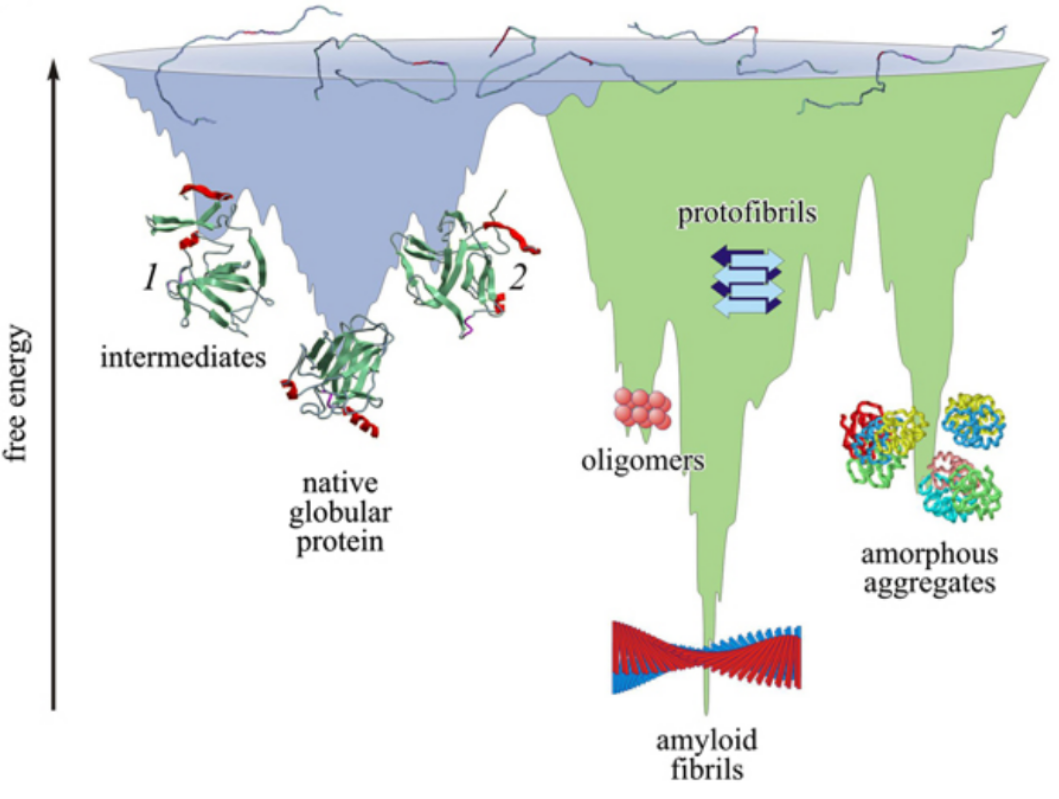
\includegraphics[width=0.7\textwidth]{img/globularEnLandscape.png} 
\centering
% 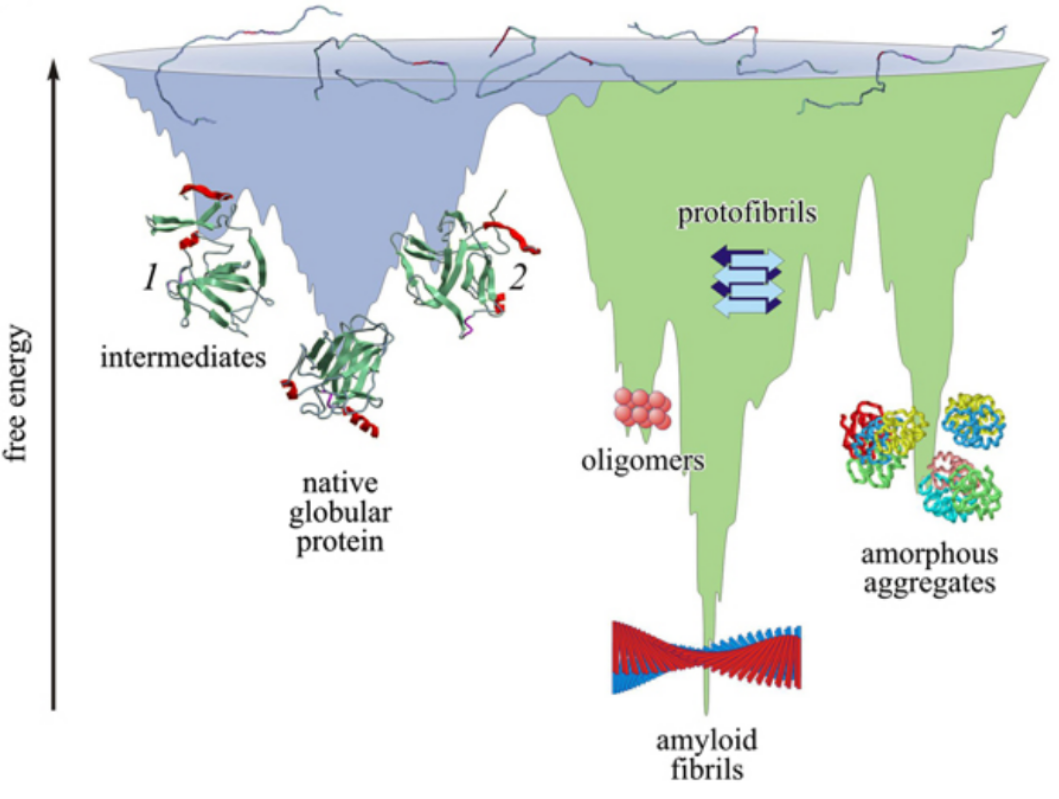
\includegraphics[width=0.7\textwidth]{img/globularEnLandscape.png} 
\caption{Perfil energetico de los estados de un polipeptido con estructura nativa globular. Figura extraida de \cite{turoverov2010protein}}
\label{globularFullEnLandscape}
\end{subfigure}

\begin{subfigure}[htbp]{\linewidth}
\centering
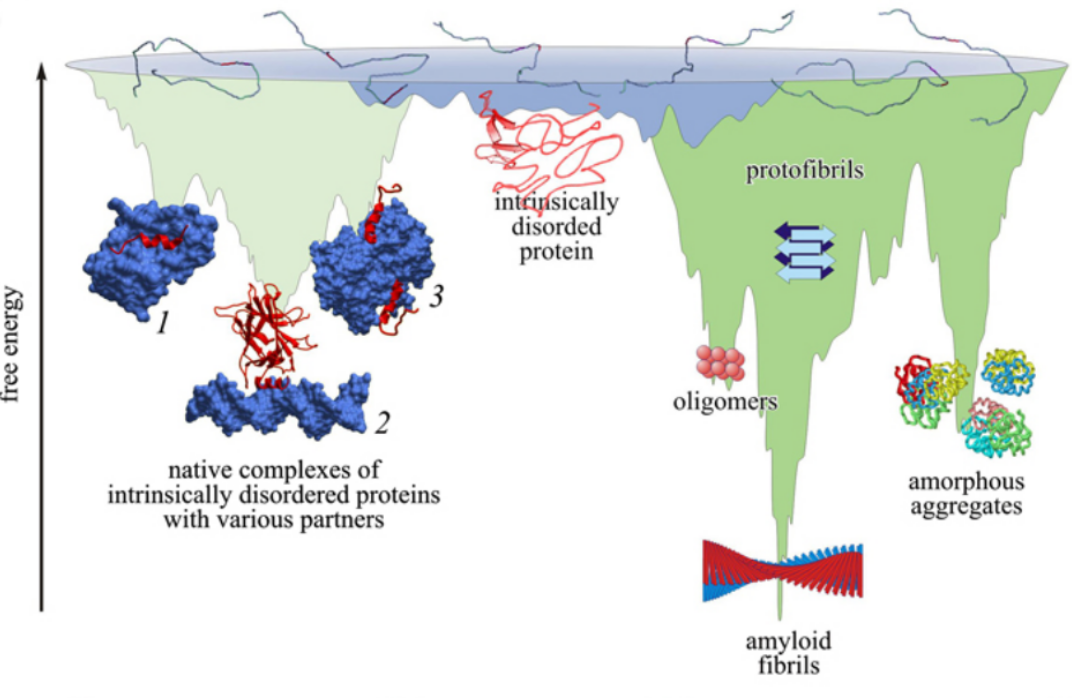
\includegraphics[width=0.7\textwidth]{img/idpEnLandscape.png} 
\caption{Perfil energetico de los estados de un polipeptido con estructura nativa desordenada. 
Disordered segments of these proteins can gain ordered structure at the interaction with specific binding partners in a case if the free energy of such complexes is lower 
than the free energies of the intrinsically disordered protein and its partner. 
1, 2, and 3 represents native complexes of intrinsically disordered proteins with various partners.
Por si solo, el polipeptido presenta a relatively flat energy landscape(sección central). Figura extraida de \cite{turoverov2010protein}}
\label{idpFullEnLandscape}
\end{subfigure}
 \caption{Full energy landscape}
 \label{fullEnLandscape}
\end{figure}


% BARRERAS CINETICAS QUE IMPIDEN LA FORMACION DE AMYLLOIDS
Provided that the native
state is maintained under conditions where it remains
folded, aggregation to amyloid fibrils will be resisted by
the kinetic barrier associated with unfolding, even if the
aggregated state is thermodynamically more stable.
% Importantly, the cooperative nature of protein structures
% means that virtually none of the polypeptide chain in individual molecules is locally unfolded, 
% and that virtually no
% molecules in an ensemble are globally unfolded, even
% though native proteins are only marginally stable relative
% to denatured ones under normal physiological conditions


An analysis of a series of amyloid fibrils suggests that
these types of structure are likely to become thermodynamically unstable relative to globular native structures, and indeed even relative to unstructured states, for
polypeptide chains of more than ~150 residues because
of the topological constraints that are associated with the
packing of a long polypeptide chain into the fibril core (REF: Metastability of native proteins and the phenomenon of amyloid formation).
Biology may have exploited this feature by evolving proteins with 300-500 residues on average to minimize the
risk of amyloid formation. 

In accordance with this view,
the amyloid fibrils that are known to be associated with
disease are all composed of relatively short peptides or
proteins, or of proteolytic fragments of larger precursor
proteins (TABLE 1) .

















These observations, therefore, have led to the remarkable conclusion that,
at the concentrations present in living systems,
the native states may not always represent
the absolute free energy minima of the corresponding polypeptide chains, the native form of a protein could in some cases simply be a metastable monomeric
(or functionally oligomeric) state that is separated from
its polymeric amyloid form by high kinetic barriers.
As much evidence reveals that the amyloid state is
very resistant to denaturants and proteases, and mechanically robust, such a state could represent, at least under
some conditions, a highly structured alternative to the
native state but one that under normal biological conditions, although not under some disease-associated ones,
may be kinetically inaccessible. 
Understanding such kinetic factors therefore becomes a major target for developing an understanding of the circumstances in which
amyloid assemblies occur in living systems.






% **************************************************
% CONCLUSION SOBRE ESTADOS CONFORMACIONALES  -------   NO SE DONDE PONER ESTO!!! 
% *******************************************************
Es por esto que las propiedades conformacionales de una proteína quedan mejor definidas si se declara el conjunto de multiples estados accesibles por sus estructuras.
A este continuo de conformaciones que pueden adoptar las proteinas individuales, se agregan distintos tipos de estados agregados, conformados a partir de uniones entre proteinas 
en distintas conformaciones iniciales(conformaciones desestructuradas, intermedios o plegados).
De acuerdo con esta forma de ver, esta accesibilidad estará dada por la estabilidad termodinámica de cada conformacion accesible y la cinética de interconversión entre estas.
% Estos requerimientos pueden indicar por ejemplo q ciertos estados altamente estables como puede ser las fibras amiloides no sean estados naturales comunes debido a los requerimientos cinéticos, a pesar de ser termodinamicamente estables.
% De acuerdo con esta forma de describir las posibles conformaciones de las proteinas, the various fates awaiting a polypeptide chain once it has been synthesized in the cell 
% will depend on the kinetics and thermodynamics of the various equilibria between di¡erent possible states.

Las propiedades cinéticas y termodinámicas están dadas por el contexto celular (pH, iones, concentracion de proteinas, presencia de otras moleculas con las que interactúa, etc) y, 
obviamente, por los posibles cambios que puede tener una proteina, ya sean mutaciones o modificaciones postraduccionales.
Esta forma de ver las propiedades estructurales permite ver los origenes de los cambios conformacionales desde el punto de vista de las propiedades fisicoquimicas de las proteinas.
If the stability or cooperativity of the native state of a protein is reduced, for example by a mutation, the population of non-native states will increase.
Es importante destacar, entonces que, for a given polypeptide chain a chosen fate is not a final one, and a choice may be further modulated by environmental pressure. 
Thus, intrinsically unstructured proteins may be forced to fold or misfold via modification of their environment (addition of natural binding partners, changes in properties of solvent and so on), 
whereas a destabilizing environment may push a natively folded protein to the misfolding route. Alternatively, the presence of chaperones may reverse the misfolding route and effectively dissolve small aggregates
To begin to understand the manner in which proteins either adopt and maintain the specific states that are needed to carry out given functions or instead misfold
and form potentially pathogenic aggregates such as amyloid fibrils, it is important to investigate the nature and properties of the various states in which these molecules
can be found. 
It is also important to clarify how the conversion of proteins into the amyloid state(o cualquier estado no funcional) is generally avoided in living systems.  
% *****************************************************************************
%ESTO ES LO QUE SE ESTUDIA A CONTINUACION  !!!!!!!!!!!!!!!!!!!!!!!!!!!!!!!!!!!!!!!!!!!!!!!!!!!!!!!!!!!!!!!!!********************
% 




















% EL PROCESO Y LA CINETICA DE LA FORMACION DE FIBRAS AMYILOIDS

% REF:  Protein aggregation: Mechnisms and functional consequences
% Amyloid fibrillogenesis is usually modelled as a nucleation-elongation polymerization process, which reaction rate depends on the protein concentration and can be accelerated 
% by the addition of homologous pre-aggregated polypeptides that act as seeds/templates promoting the transition from the soluble to the aggregated state
% According to this simplified model, amyloid aggregation can be divided in three main phases: 
% (1) The thermodynamically dis-
% favoured lag phase where the soluble species (usually monomers)
% associate to form nuclei, a poorly characterized state which for-
% mation influences the overall kinetics of the amyloid reaction. (2)
% The population of these transient assemblies triggers the poly-
% merization and fibril growth at the so-called exponential phase.
% (3) Finally, the exhaustion of monomers leads to the saturation
% phase where no more soluble species can associate to the ends of
% preformed fibrils and fibril maturation occurs, usually by lateral
% association of fibrils








% ***********************************************
% DEPENDENCIA DE LA AGREGACION CON LA SECUENCIA
% ***********************************************
Even though the ability to form amyloid fibrils seems to be generic(is a general property of the polypeptide backbone), 
the propensity to do so under given circumstances can vary markedly between different sequences(depends enormously on amino acid composition.).

The question of how amino acid composition influences aggregation propensity is highly relevant to protein design, as well as
to our understanding of protein evolution and the pathogenicity of certain amino acid substitutions.
Ademas, funciona como base para el desarrollo de herramientas bioinformaticas que permitan detectar secuencias con tendencia a formacion de agregados


% DEPENDENCIA CON LA COMPOSICION
Given the fact that hydrophobic
interactions are a major driving force of protein self-assembly, it is
expected that increased hydrophobic content in a peptide would
lead to increased aggregation propensity, while a net charge on
the peptide would impede aggregation. Also, with the evidence
for common cross-b architecture among amyloid fibrils of diverse
proteins (Nelson et al., 2005), a stretch of amino acids with
enhanced propensity to adopt b-strand secondary structure
would be expected to promote formation of fibrils. Such physico-
chemical properties of amino acids are the basis of most of the algo-
rithms that predict either the rate or propensity of aggregation of
different regions of a protein .  %****ESTO SE CONTINUA EN LA SECCION HERRAMIENTAS 

La relacion entre estas propiedades(hidrofobicidad, carga neta, tendencia a formar $\beta$) se analiza en  \cite{chiti2003rationalization} utilizando mutaciones sistematicas sobre polipeptidos,
encontrándose que ... the propensity of a  given  polypeptide  chain  to  aggregate  under  specific  conditions varies  dramatically  with  its  composition  and  sequence.
These results show how the primary structure of proteins plays an extremely relevant role in determining the tendency of polypeptides to form insoluble deposits;
this would arise from the impact over such propensity of inherent physical-chemical properties of amino acids such as hydrophobicity, the
structural suitability to adopt $\beta$-conformation or its mean charge

The aforementioned factors may be regarded as intrinsic determinants arising
from individual properties of amino acids. Nonetheless, the linear combination
of their properties along the primary structure has a cooperative impact over the
aggregation propensity. 
% It has been observed that the consecutive occurrence of three
% or more hydrophobic residues is clearly disfavored in nature [29]. In a similar way,
% the combinatorial design of amyloidogenic proteins has shown how polypeptidic
% patterns alternating apolar and polar aminoacids favor amyloid formation [30].




% DEPENDENCIA CON SEGMENTOS DE SECUENCIA
The intrinsic determinants described before inform us about specific properties of the amino acid side chain either favoring or disfavoring protein aggregation.
The linear combination of such properties within the primary structure plays a major role in protein aggregation.
However, it has been observed that not all the polypeptide sequence has the same importance in defining its propensity to aggregate. 
En \cite{ventura2004short} se demuestra que ....
There exist small amino acid stretches within protein sequences, which promote and guide protein aggregation into amyloid-like structures
These short fragments, generally referred to as aggregation-prone regions (APRs) or “hot-spots”, are characterized by an enrichment in hydrophobic, both aliphatic (Val, Leu,
Ile) and aromatic (Phe, Trp, Tyr), residues.
The analysis of the structural models for some amyloids also allow to rationalize the reason why APRs direct the formation of amyloid-like structures, since the cross-$\beta$ arrangement in the core of
amyloid fibrils does only strictly require the minimum participation of a single $\beta$-strand per molecule, and the rest of the polypeptide may remain exposed to the
solvent even when “attached” along the fibril.

 most of the natively unfolded proteins in vivo do not undergo aggregation (13), indicating that unfolding is necessary, but not sufficient, to promote aggregation. 
Hence, there must be some sequence motifs that, once they become exposed, are more prone to aggregation than others. 
In fact, experimental evidence is compelling in favor of the hypothesis that small regions of a protein are responsible for its amyloidogenic behavior

% Although all proteins can form amyloid fibrils under the appropriate conditions, the list of currently known trouble 
% makers  (i.e.,  proteins  aggregation  of  which  is  directly  responsible  for  the  development  of  various  pathologies)  is  rather  short, including 30-40 proteins and protein fragments.
% Why  do some proteins form fibrils under the  physiological conditions, whereas others do not? 
% It is clear now that frequently not entire protein is responsible for aggregation and rather aggregation 
% is driven by specific  protein  regions  that  contains  specific  structural  or  sequence  motifs,  so-called aggregation-prone  regions,  APRs, which contribute significantly toward the overall aggregation propensity of the protein
% 



% FACTORES EXTERNOS QUE AFECTAN LA AGREGACION
Además de las propiedades que se analizaron sobre la secuencia primaria, es importante destacar factores externos a la secuencia que pueden afectar la formación de agregados.
The most relevant extrinsic determinants are the pH and
the ionic strength of the solution, together with the temperature of the system [34].
These variables may affect both the kinetics and thermodynamics of aggregation
into amyloid-like structures, and can, subsequently, influence the assembly and
the macroscopic structure of the aggregated species, thus being important deter-
minants of the polymorphism the aggregates of a given protein sequence may
present.











% % FUNCTIONAL AMYLOIDS
% Contrary to amorphous aggregates, amyloid structures can fulfill biological functions, and functional amyloids are found in organisms from prokaryotes to humans \cite{fowler2007functional}.
% % 
% Amyloids are not only associated with disease-related proteins.
% Nature also exploits the structural and mechanical properties
% of amyloids to regulate biological functions 13 . For example, in
% bacteria amyloids such as curli promote biofilm formation and
% host invasion, and chaplins in bacteria and hydrophobins in yeast
% act as regulators of surface tension of water. Insects and fish
% use chorion amyloid as a component of eggshell, and spiders
% use spidroins in spider silk. Humans possess at least one func-
% tional amyloid protein: Pmel17 is used as a structural scaffold
% in melanin synthesis. The strength and flexibility of amyloids
% have attracted attention for their use as biomaterials. However,
% it remains to be understood how functional amyloids avoid the
% cytotoxic effects observed in disease amyloids. In part, functional
% amyloids are regulated by chaperones and proteases. But it is
% also becoming evident that sequence composition modulates
% critical biophysical parameters determining kinetics of assembly
% or mechanical strength.






% Las fibras amiloides se consideran que estan asociadas to more than 40 human pathologies, esto generó un gran interés en estudiar sus propiedades, 
% las formas detectar secuencias con tendencia a formarse y las formas de prevenir su formación in vivo.
Despite active research, a detailed understanding of the molecular principles underlying the transformation of soluble proteins into amyloid aggregates is still lacking

Since all fibrils independent of the original structure of the given amyloidogenic protein have a common cross-b structure, considerable conformational rearrangements have to occur prior to fibrillation. 
Such changes cannot happen in a native protein, due to its stable and rigid tertiary structure. Thus, protein destabilization favoring partial unfolding and culminating in the formation of a partially unfolded conformation is required. 
Presumably, such a partially unfolded conformation favors reciprocal and specific intermolecular interactions, including electrostatic attraction, hydrogen bonding and hydrophobic contacts, which are necessary for oligomerization and fibrillation
Obviously, this model does take into account a class of natively unfolded proteins, as they are devoid of rigid tertiary structure in their native state.

% Data have been reported indicating that the first critical step in protein fibrillogenesis is the partial unfolding of the protein. 
% Due to structural fluctuations (conformational breathing) the structure of a globular protein under physiological conditions represents a mixture of tightly folded and multiple partially unfolded conformations, 
% with great prevalence of the former. 
% Most mutations associated with accelerated fibrillation and protein deposition diseases have been shown to destabilize the native structure, increasing the steady-state concentration of partially folded conformers

% En la mayoria de las proteinas, excepto las mas pequeñas, el 'unfolding' que ocurre en condiciones fisiologicas no lleva a una estructura totalmente desplegada sino que la proteina adquiere una estructura semi-estable parcialmente collapsada,
% donde las interacciones no son las mismas que en el estado nativo estructurado, estas son caracteristicas propias de los intermediarios del plegamiento.

% The energy landscape model suggests that some folding intermediates might have structural elements not present in the final folded state(en el estado final pueden estar metidas en el centro hidrofobico).
% The appearance of such misfolded intermediates might initiate protein oligomerization or aggregation.

% La formacion de estos intermediarios es importante porque generalmente son mucho mas solubles que si se formaran conformaciones altamente desplegadas. 
% Esta solubilidad permite alcanzar las concentraciones requeridas para la nucleacion propia de la formacion de amyloids(y de agregados en general????)

% Detailed structural analysis of early fibrillation events in several proteins has demonstrated that the amyloidogenic conformation is only slightly folded and shares many structural properties with the premolten globule state.

% This picture enables us to speculate on the origins of the amyloid diseases from the point of view of the physico-chemical properties of the protein molecules. 
% If the stability or cooperativity of the native state of a protein is reduced, for example by a mutation, the population of non-native states will increase.
% This rise will increase the probability of aggregation, as the concentration of polypeptide chains with at least partial exposure to the external environment will be greater. 

Whether or not aggregation does occur will depend on the concentration of protein molecules, the intrinsic propensity for a given sequence to aggregate when unfolded, and on the rate of the aggregation process. 
The fact that formation of ordered amyloid fibrils can be seeded, like the well-studied processes of crystallization
and gelation, means that once the aggregation process is initiated it often proceeds very much more rapidly.
In the absence of seeding there can be long 'lag' phases before aggregation occurs . 
This lag can be thought of as arising because the growth of a fibril cannot occur until a 'nucleus' of a small number
of aggregated molecules is formed. 

Such a nucleus can be formed by the local fluctuations in concentration that occur in solution as a result of random molecular motion. When such fluctuations result in a local concentration of
molecules above a critical value, the molecules associate with one other to form a species that is suficiently large to have intrinsic stability, and hence to grow in size by interacting with other molecules in the solution. The act
of seeding provides such nuclei to the solution and hence reduces or abolishes the lag phase

The proposal that amyloid fibrils are a generic structure of polypeptide chains (lo que los hace genericos, que se desarrollo antes) coincide con este modelo de formación.











% ACA EXPLICO POR QUE LAS IDPs NO TIENEN TANTA TENDENCIA A FORMAR AGREGADOS
In contrast to the globular proteins, which have to unfold prior to aggregation, IDPs are always ready for intermolecular interactions. 
An unbound fragment of an IDP possesses a strong ability to interact, and therefore can bind either to natural partners forming native complexes or to similar molecules forming various aggregates. 
This raises the question of why IDPs do not always form aggregates in the norm. One of the potential answers is the fact that inside the cell, the IDPs typically form complexes with natural partners.
Los mecanismos de proteccion (chaperonas, proteasoma, etc) tienen una gran capacidad para mantener la solubilidad de proteinas.
Además, based on the analysis of the IDP amino acid composition, it would be clearly a mistake to assume that an averaged IDP possesses higher propensity towards aggregation than an averaged ordered
protein. In fact, many IDPs contain large number of charged and polar residues. In addition to the hydrophobic interactions, the net charge is one of the major factors determining aggregation behavior of a protein.

En \cite{linding2004comparative} se hace un estudio interesante de comparación entre un set de proteinas que adoptan estructuras globulares y otro que experimentalmente se sabe que son IDPs.
Se hace el analisis usando TANGO

Intrinsically disordered proteins are not necessarily prone to aggregation, as their sequences have usually evolved to maintain the level
of solubility that is required for their optimal function; for example, through the existence of extensive regions that are highly abundant in charged and polar groups
that disfavour intermolecular association from a thermodynamic point of view. 
Moreover, as is discussed below, kinetic barriers to aggregation are crucial in enabling both globular and disordered proteins to maintain their soluble and functional states.

























% 
% 
% 
% ***********************************************************
% CON LOS PROXIMOS PARRAFOS ARMAR UNA
% CONCLUSION GENERAL SOBRE TODOS LOS ESTADOS DE AGREGACION
% ************************************************************
% 
% 


% ACA DIGO QUE LAS FIBRAS AMILOIDES NO SON LA UNICA ESTRUCTURA PRODUCTO DE MISFOLDING
% 
% % PUEDO APROVECHAR ESTE PARRAFO PARA EXTENDER LA IDEA QUE LOS AGREGADOS NO SON NI 1 NI 2 Y QUE PUEDE HABER UNA GRAN CANTIDAD DE FORMAS EN LAS QUE SE AGREGAN LAS PROETEINAS
% En \cite{narhi2012classification} se estudian distintas formas de clasificación de agregados de proteínas:
% Protein aggregation is a complicated phenomenon,
% which is sensitive to solvent conditions, sample his-
% tory, protein sequence, and so on. Our ability to un-
% derstand aggregation will depend on the identifica-
% tion of patterns within this vast parameter space. It
% is our hope that these patterns will be more appar-
% ent with a more precise naming scheme. We propose
% using five categories: size, reversibility/dissociability,
% conformation, chemical modification, and morphol-
% ogy, to consistently describe protein aggregates.


% De todos los posibles estados de agregación, nos centramos en la formación de fibras amiloides porque....
% % Esto esta en \cite{knowles2014amyloid}
% The amyloid state, however, is relevant not only in
% the context of disease, but also because its very existence
% challenges in many ways our current understanding of the
% nature, structure and evolution of the functional states of
% proteins 26–30 . From a wide range of in vitro experiments on
% peptides and proteins we now know that the formation of
% amyloid structures is not a rare phenomenon associated
% with a small number of diseases but rather that it reflects a
% well-defined structural form of the protein that is an alter-
% native to the native state — a form that may in principle be
% adopted by many, if not all, polypeptide sequences









% MERGEAR ESTE PARRAFO CON EL QUE SIGUE, ARMANDO UNA CONCLUSION

% Although the data presented above were mostly devoted to a consideration of 
% protein fibrillation, the process of amyloid fibril formation does not represent the only misfolding route. 
% in fact, contrary to the process of productive protein 
% folding leading to the appearance of a rigid conformation with the specific 
% function, the end products of misfolding may have a different appearance. The 
% morphology of these end products depends on the particular experimental 
% conditions, and misfolded product may appear as soluble oligomers, amorphous aggregates, or amyloid-like fibrils. 
% any of these three species could be 
% cytotoxic, thus giving rise to the development of pathological conditions. 
% The reason for such a morphological difference is potentially connected with the diversity of the partially folded intermediates favoring protein self-association. 
% In fact, multiple environmental factors, such as point mutations, decrease in pH, increase in temperature, the presence of small organic molecules or metal ions, and other charged molecules, might induce structural rearrangements within a protein molecule, shifting equilirium toward the partially folded conformation(s). As different factors may stabilize slightly different partially folded intermediates, the formation of morphologically
% different aggregates is expected.













































\subsubsection{Mecanismos naturales de proteostasis}



%  En \cite{balch2008adapting} se hace un desarrollo bastante completoo de los mecanismos de homeostasis
The  obvious  consequences  of  misfolding  are protein  aggregation  (and/or  fibril  formation),  loss  of  function,  and  gain  of  toxic  function.  
In  order  for  any  biological  system  to  function  effectively,  it  is essential to avoid the inherent tendency of proteins to aggregate and form potentially harmful deposits.
It  is  clear (a partir de lo que se dijo en la seccion anterior)  that  the aggregation  process  is  generally   initiated  from  partially  or completely  unfolded  forms  of  the  peptides  and  proteins. 


Como se vió en las secciones previas, el espacio de conformaciones accesibles por las proteinas dependia de las estabilidades termodinamicas de los estados y la cinetica de interconversión entre estos. 
Estas propiedades, a su vez, dependen del contexto celular en el que se encuentran(ademas de la secuencia de la proteina en si misma), concentraciones de proteinas, localizacion, interacciones, etc.
The healthy state of a cell is characterized by a detailed balance between the different states that proteins can populate. 
Perturbations to such balance, unless they are kept under strict control, can lead to deleterious events and disease.
El balance correcto entre todas estas condiciones está regulado a traves del proceso de proteostasis.
Proteostasis refers to controlling the concentration, conformation, binding interactions (quaternary structure), and location of individual proteins making up the proteome by readapting the innate biology of the cell, 
often through transcriptional and translational changes.
% The protein components of eukaryotic cells face acute and chronic challenges to their integrity. Eukaryotic protein homeostasis, or proteostasis, enables healthy cell and organismal development and aging and protects against disease
% Los mecanismos dentro del proceso de proteostasis permiten successful organismal development and aging in the face of constant intrinsic and environmental challenges %previniendo el desarrollo de enfernedades.
La proteostasis es influenciada por todos los mecanismos que controlan los aspectis vistos en las secciones previas..... 
by the chemistry of protein folding/misfolding and by numerous regulated networks of interacting and competing biological pathways 
that influence protein synthesis, folding, trafficking, disaggregation, and degradation.

La celula posee distintos mecanismos para regular estos procesos .....chaperonas para regular el proceso de folding/misfonding (y tambien de aggregation), 
Nature developed very sophisticated protection mechanisms (chaperones, proteasome, etc.) for the effective regulation of the folding process, y por lo tanto prevenir las peligrosas consecuencias de misfolding. 
In other words, in the cell, any given protein is not acting in the isolation, is never alone and is constantly "watched" by the protective machinery. This machinery is rather robust and can
tolerate significant loads. Obviously, factors that affect these protective mechanisms will contribute to the probability of disease development

% MECANISMOS CELULARES
En \cite{gsponer2012cellular} se desarrollan una gran cantidad de mecanismos celulares que ayudan a prevenir la agregacion de proteinas. 
Se demuestra que aggregation-prone proteins are subject to differential transcriptional, translational, and degradation control compared to nonaggregation-prone proteins, which leads to their decreased
synthesis, low abundance, and high turnover. 

% PROPIEDADES INTRINSECAS DE LAS PROTEINAS
Como se vio en las secciones previas, as proteins in their functional forms can be thermodynamically and chemically metastable, mechanisms have evolved to maintain their solubility in vivo for prolonged periods of
time and to avoid their conversion into non-functional amyloid states.
En \cite{knowles2014amyloid} se muestran varias propiedades de estos mecanismos. 
Es decir, además de los mecanismos dinámicos que se encuentran en la celula y que, generalmente, se adaptan a las señales del entorno celular, existen propiedades evolutivas para mantener estados de proeostasis.
Algunos de estos son:
-APRs are usually located within or substantially take part in the hydrophobic cores of the native state of proteins [39] and also frequently map to protein-protein interaction surfaces of protein adopting
a stable quaternary structure [40, 41], which prevents APRs from establishing aberrant intermolecular contacts

-The examination of APRs in the context of entire proteins has also revealed how these stretches are usually flanked by charged residues (Asp, Glu, Lys, Arg), whose
function would be to hamper intermolecular interactions between APRs in the event they become exposed by providing repulsive charge, or by residues acting as $\beta$-sheetbreakers, like Pro


IDPs play a central role in many cellular processes, as their disordered nature provides them with the ability to bind many partners, thereby regulating many biochemical
processes. Because of this central role, the malfunction of IDPs can disrupt proper cellular function and lead to disease.

% Las diferencias estructurales vistas entre los distintos estados de agregación tambien se ven reflejada en diferencias biológicas 
% Whereas misfolded and aggregated proteins are found in perinuclear locations and are generally degraded by the 
% proteasomal system, amyloids preferentially accumulate in perivacuolar inclusions, where they are degraded by the autophagosome.

Esta segregación resulta en un tratamiento distinto por parte de los mecanismos encargados de la proteostasis.
A reduced affinity of amyloids for the protein quality control system is probably also at the root of their higher toxicity 11 as artificial overexpression of chaperones
usually leads to decreased toxicity and removal of amyloids from he cell.





% PREVENCION DE AGREGACION EN FOLDED PROTEINS
% the normal folding process may pass through
% partially folded states on the route to the fully native state,
% but the aggregation of these species will be minimized by
% the presence of molecular chaperones. In addition, if the
% protein is able to fold rapidly, any partially folded species
% will have a short lifetime, reducing the probability of inter-
% molecular interactions occurring. Moreover, once folded,
% the native state is generally a highly compact structure
% that conceals the polypeptide main chain within its
% interior. Such a state is protected from aggregation except
% through the interactions of surface side chains (as is the
% case, for example, in protein crystals) and is unable to
% form the strong intermolecular hydrogen bonds associated
% with the polypeptide backbone. 














































































\subsection{Características/elementos funcionales}
\label{functionalLandscape}


% PARADIGMA ESTRUCTURA-FUNCION TRADICIONAL 
The structure-function paradigm claims that a specific function of a protein is determined by its unique and rigid three-dimensional (3D) structure. 
Thus, following its biosynthesis on the ribosome, a protein must fold to a native, defined 3D structure to be functional. 
One of the bestunderstood functions of proteins is catalysis (i.e., enzymatic activity), which attracted much attention in the early days of
protein science and led to the elaboration of the “lock and key” model by Fisher. 
% En este caso(enzimas) la proteina provee un scaffold para el sitio activo, 
Central to this model is the notion that the correct shape of the substrate can fit into the active site of the enzyme for enabling an efficient and specific catalysis,
The primary origin of this structure-function paradigm is the “lock and key” hypothesis formulated in 1894 by Emil Fischer to explain the astonishing specificity of the enzymatic hydrolysis of glucoside multimers by different types
of similar enzymes. For a long period of time, the validity of “lock and key” model and its associated sequence-structure-function paradigm was unquestioned, especially after the crystal structures of proteins started to be solved by X-ray diffraction
Este paradigma se deriva de los primeros avances en el estudio de estructuras de proteinas. Over the past century evidence steadily accumulated that a well-defined structure is the prerequisite of protein function.
Basic biology and biochemistry textbooks that explain biological phenomena at the molecular level exquisitely rely on this notion, the ‘structure–function paradigm’.
The explanatory power of these 3-D structures continued to reinforce the static view of protein

Throughout the 20th century, tens of thousands of structures have been solved and deposited in the Protein Data Bank (PDB), supporting again the necessity of a 3-D structure for functionality.
that remained unquestioned.
In contrast to this view, already in 1958 Koshland suggested the “induced-fit” model based on the observations that some enzymes could act on
differently shaped substrates and hence a degree of flexibility is inevitable in function. 
A pesar de este reconocimiento de la dinamica para la funcion biologica, con cambios conformacionales que van desde variaciones en rotameros de las cadenas laterales hasta reordenamientos conformacionales mas relevantes
(por ej. en proteinas alostericas), estas variaciones podian aun ser interpretadas dentro del modelo establecido por el paradigma estructura-funcion.
A well-folded, albeit dynamic, structure was thought to be the hallmark of protein function.

In general, such proteins are categorized as being "folded", and for these proteins(como se vio al inicio de la seccion de conformaciones), 
structures determined by experimental methods such as X-ray crystallography correspond to the ensemble-averaged structures.
Since the folded ensemble contains structures that have only small deviations from the ensemble average structure, 
the ensemble average itself captures many important features of the protein's structure, and many insights into a protein's function can be garnered from this
ensemble average structure
Es decir, dado que en dominios globulares la estructura esta definida(podemos obtener un ensemble avarage) y esta asociada a la funcion que desarrolla la proteina, 
% esta estructura puede ser usada para clasificacion y para inferir la funcionalidad en nuevas proteinas.
Estos dominios globulares pueden ser identificados y asociados a una funcion individual o a una funcion dentro de la funcion global de la proteina.
% PFAM, SCOP

El paradigma secuencia-estructura-funcion permite extender este concepto a la estructura primara de la proteína.
Dado que la estructura asociada a la función debe mantenerse, los requerimientos estructurales(y funcionales) imponen, a su vez, ciertas restricciones sobre la evolución de la secuencia.
Esto facilita la anotación de funcionalidad/elementos funcionales en secuencias nuevas, aun cuando no se conoce su estructura.

Incluso cuando ....The sequences diverge, but the overall domain architecture remains the same.
Particular domains and domain architectures are well conserved over the course of evolution. 






% HASTA ACA DEBERIA HABER DEFINIDO TODOS LO QUE RESPECTA A ESTRUCTURA-FUNCION EN DOMINIOS GLOBULARES

% ARRANCO CON IDPs


However, globular domains are only part of the picture. 
Many studies have shown that they cover only a fraction of the protein sequence contained in an organism. 
Como se vio en la primera sección, las conformaciones nativas de las proteinas pertenecen a un continuo de conformaciones y multiples evidencias indican, independientemente, 
que una proteina pueden existir simultaneamente en distintas conformaciones.


% ACA YA SE SOBREENTIENDE QUE LAS IDPs/IDRs PUEDEN TENER FUNCIONALIDADES


% Protein sequences in a genome can be viewed as modular because they are made up of combinations of structured and disordered regions.
% Proteins without IDRs are called structured proteins, and proteins with entirely disordered sequences that do not adopt any tertiary
% structure are referred to as intrinsically disordered proteins (IDPs). 
% The majority of eukaryotic proteins are made up of both structured and disordered regions, and both are important for the
% repertoire of functions that a protein can have in a variety of cellular contexts.

% Thus, functional regions in proteins can
% either be structured or disordered, and these need to be
% considered as two fundamental classes of functional building
% blocks of proteins





Como se dijo en la introduccion, a little more than 10 years ago,however, such challenge to the almost dogmatic ‘structure–function paradigm’ was pure heresy due to the overwhelming evidence that structure determines function.
As it is often the case for new scientific concepts, the idea of structure-less functionality went through the stages of passive ignorance and active denial to scrupulous examination and enthusiastic acceptance
Como parte de estos avances, en los ultimos años se han encontrado gran cantidad de proteinas que adoptan estructuras cuyas conformaciones son total o parcialmente desordenadas(segmentos globulares), soportando esta definicion, formalizada a principios de milenio. 
the transition in paradigm was enforced by scattered experimental observations of disorder in a few dozen proteins. 
Evidence added to that obtained by other techniques [mostly NMR and circular dichroism (CD)]..... and the evidence seems overwhelming now that structural disorder also exists in vivo and it is truly the native, functional state of these proteins.
A decade of steady progress turned skepticism around and the suggestion that the native state of many proteins is intrinsically disordered (or, as originally termed, unstructured) is now integral to our general view of protein structure and function.
% una de las dudas que se tenia era si este estado conformacional existia solo in vitro y en realidad in-vivo lo que ocurria era que el crowding generaba el plegamiento

\begin{figure}[h!,centered]
\centering
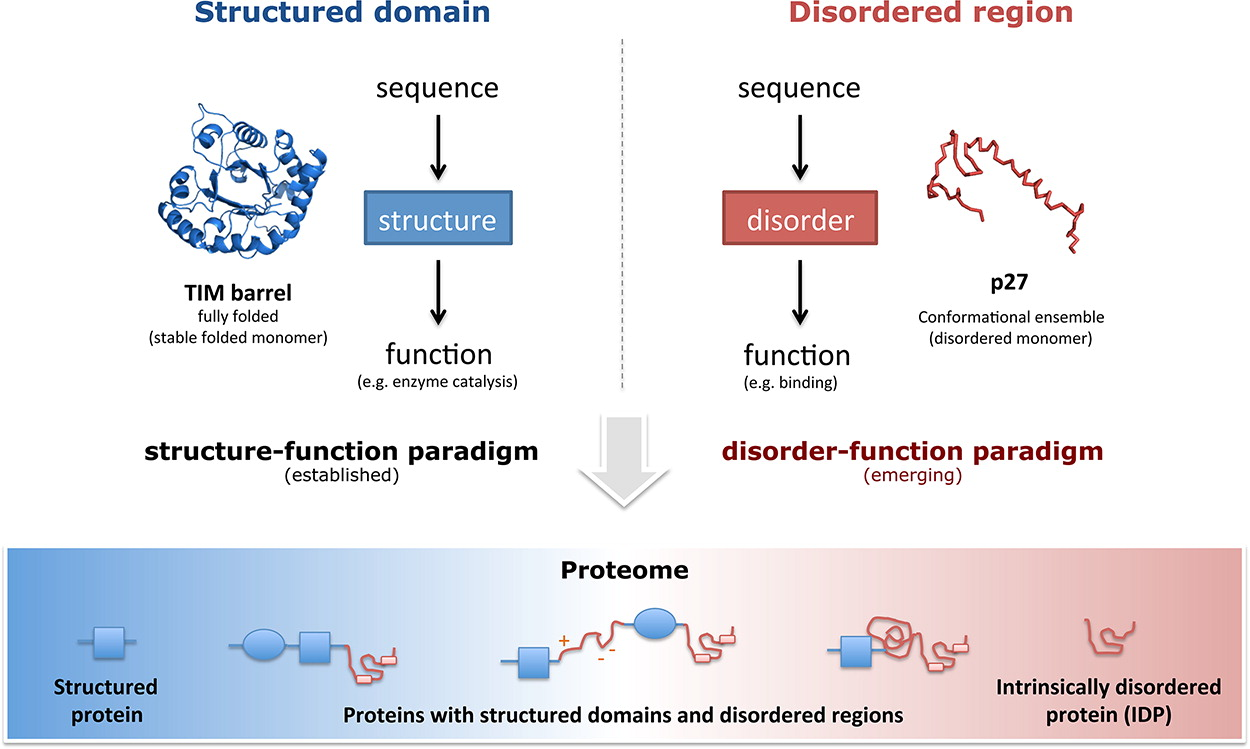
\includegraphics[width=0.9\textwidth]{img/structure-idp-function.jpeg} 
\caption{Paralelismo entre funcionalidad emergente de dominios plegados y de proteinas IDPs. Figura extraida de \cite{van2014classification}}
\label{stuctured-idp-functions}
\end{figure}


These proteins challenge(o mejor dicho destruyen) the “one sequence—one structure—one function” concept by demonstrating that the lack of stable tertiary and/or secondary structure does not preclude proteins from being biologically active
As the main criterion of a native protein is its ability to perform a biological function, these partially or completely disordered proteins must be regarded as native entities.
This means that the structure-function paradigm, which emphasizes that ordered 3D structures represent an indispensable prerequisite to effective protein functioning, should be redefined to include intrinsically unstructured proteins. 
According to this redefined paradigm,  native proteins (or their functional regions) can exist in any of the known conformational states.
El proteoma funcional esta compuesto, entonces, de un continuo de conformaciones que fall onto a structural continuum, from tightly folded single domains, to multidomain proteins that might have flexible or disordered regions, 
to compact but disordered MOLTEN GLOBULES and, finally, to highly extended, heterogeneous unstructured states \ref{stuctured-idp-functions}




% PROTEIN QUARTET 
% PUEDO SACARLO COMPLETAMENTE
% 
% 
% To accommodate all these states in a functional framework, was elaborated the protein trinity hypothesis \cite{dunker2001protein} ,
% which posits that a native protein can be in one of three states -the ordered state, the collapsed-disordered (molten globule, MG) state, and the extended-disordered state (random coil, RC)- and that function can arise from any of the
% three states or from transitions between them. This model was subsequently expanded to include the premolten globule (PMG) state, which corresponds to an intermediate state between the RC and the MG. \ref{proteinQuartet} 
% % El modelo resultante actual esta compuesto de 4 estados\ref{proteinQuartet} que indican los posibles estados nativos(funcionales) de las proteinas.
% 
% 
% \begin{figure}[htbp]
% \centering
% 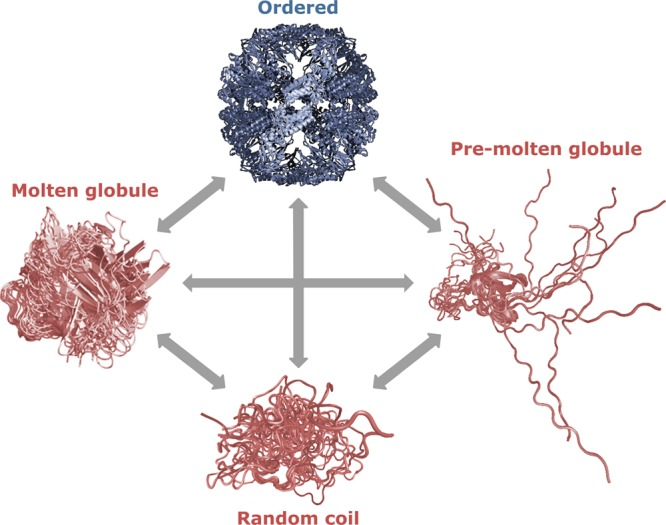
\includegraphics[width=0.7\textwidth]{img/proteinQuartet.jpg} 
% \caption{Protein quartet model of protein function. 
% Function can arise from four different conformations of the polypeptide chain, or from transitions between any of the states. Imagen extraída de \cite{uversky2002natively}}
% \label{proteinQuartet}
% \end{figure}







% PROPIEDADES Y MECANISMOS FUNCIONALES

The ultimate goal of the structural description of IDPs is to elucidate and rationalize the types and modes of functions they play.
The most important question of the field, therefore, is the physiological function and functional mode of IDPs/IDRs.


El estudio de las funcionalidades provistas por IDRs y IDPs se ve dificultada por las propiedades intrínsecas de estas proteinas:

Como se dijo antes, el paradigma inicial de secuencia-estructura-funcion provee una base para relacionar los conocimientos entre mediante metodos de analisis y anotaciones de secuencias estructuras y funciones 
By contrast, proteins within the more recently class of intrinsically disordered proteins (IDPs) sample dissimilar conformations during their biological lifetime, and therefore the corresponding structural
ensembles are heterogeneous. Given the vast number of structural states that are accessible to a disordered protein, the ensemble averaged structure for an IDP is typically not representative of any structure in 
the ensemble itself and therefore has little utility for understanding that protein's function.

Given the absence of structural constraints, IDRs tend to evolve more rapidly than protein domains that adopt defined structures. 
As a result, identifying homologous regions is harder for IDRs and IDPs than it is for structured domains.
This complicates the transfer of information about function between homologues and thus the prediction of function of IDRs and IDPs.

these considerations raise the need to devise a classification scheme specifically for disordered regions in proteins that may enhance
the function prediction and annotation for this important class of protein segments.

Aun cuando las propiedades a clasificar no sean discretas sino que formen un continuo de opciones, es util para explicar y entender mejor los conceptos.
En secciones anteriores(mas precisamente en la seccion sobre propiedades conformacionales) se hicieron clasificaciones sobre la estructura global de la proteinas/regiones desordenadas, 
ademas se clasificaron los mecanismos de binding en este tipo de proteinas como conformational selection and induced folding
Especificamente se hablara aqui de clasificaciones sobre las funcionalidades y mecanismos funcionales provistos por estas proteinas.

Como parte de estos avances para intentar dilucidar las funcionalidades de las IDPs y sus mecanismos asociados, se han intentado organizar y clasificar las funcionalidades provistas por estas \cite{van2014classification}.
En la figura \ref{proteinMechanisms} se ve una clasificación general bastante simplificada de los roles y mecanismos funcionales generalmente provistos por los distintos tipos de proteinas. 
En esta clasificacion de proteinas segun su rol general, se incluyen también los dominios/proteinas plegadas que mencionamos previamente.
La figura \ref{idpFunctions} detalla la clasificacion de funcionalidades y mecanismos funcionales específicos de IDPs/IDRs estimando las proporciones de cada funcionalidad.

\begin{figure}[h!,centered]
\centering
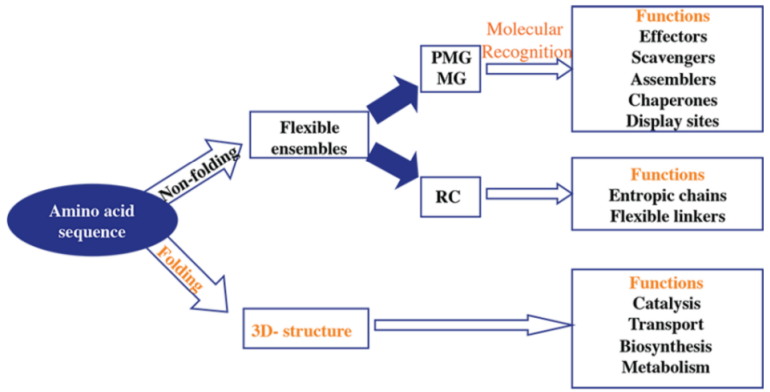
\includegraphics[width=0.9\textwidth]{img/proteinFunctionMechanisms.png} 
\caption{Distinctive properties of proteins: diversity and functional role. Figura extraida de \cite{habchi2014introducing} }
\label{proteinMechanisms}
\end{figure}





\begin{figure}[h!,centered]
\centering
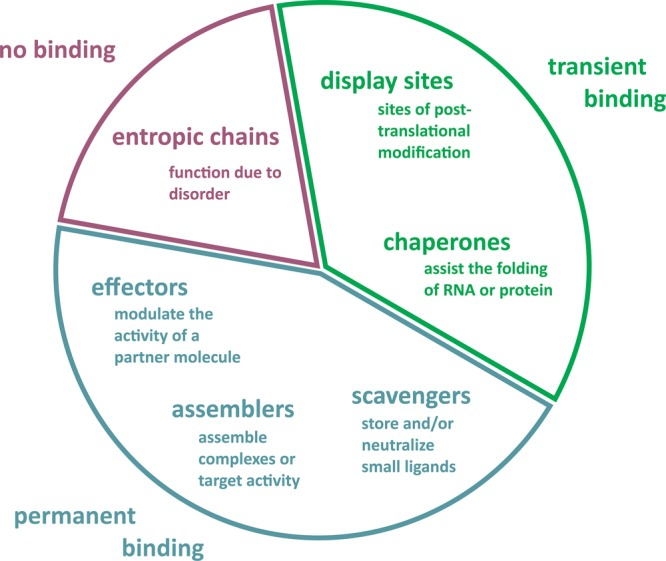
\includegraphics[width=0.7\textwidth]{img/idpFunctionMechanisms.jpg} 
\caption{Clasificación roles y mecanismos funcionales de IDPs/IDRs. Figura extraida de \cite{van2014classification}}
\label{idpFunctions}
\end{figure}


Apparent from the foregoing classification (Fig. \ref{proteinMechanisms}), IDP functions either directly stem from their disorder (((entropic chains where function involves no coupled binding and folding;
rather it directly depends on the flexibility and the plasticity of the backbone . Occupy a unique structural and functional niche in which function is a direct consequence of intrinsic disorder))), 
or from molecular recognition mechanisms , when they undergo induced folding (disorder-to-order transition) upon binding to a partner molecule. %IDPs often function via molecular recognition, when they bind partner molecules in, and induced folding process. 
Como se ve, las IDPs utilizan un mecanismo/estrategia de reconocimiento y partner binding que es basicamente diferente a la que adoptan los dominios plegados.
Mientras que estos ultimos (los dominios plegados) han evolucionado para dar una gran variedad de plegamientos diferentes que proveen reconocimientos especificos, 
el binding en IDPs is often mediated by short recognition elements (motifs)\cite{neduva2005systematic,fuxreiter2007local} de naturaleza flexible.
This mode of binding is thought to confer many advantages \cite{gunasekaran2003extended,dyson2005intrinsically}%REFERENCIA AL PAPER DE MECANISMOS FUNCIOMNALES DE IDPs



En la seccion de conformaciones, se desarrollaron conceptos relacionados con el coupled folding and binding processes.
Ahi se describio que, generalmente, only a part of an IDP, a specific recognition element, which is a relatively short amphipathic linear motif contained within long disordered sequence, is involved in the coupled folding and binding events
% Es decir, ciertos elementos funcionales 
% En relacion a este concepto, nuevos conceptos han nacido para describir este tipo de entidades biologicas,
Estos elementos funcionales, con largos de unos 10-70 amino acids, caracterizados a partir de sus propiedades conformacionales,  se denominan comunmente como Molecular Recognition Features (MoRFs)
\cite{mohan2006analysis,vacic2007characterization,oldfield2005coupled}.
Ademas, los dos modelos descritos antes sobre coupled folding and binding process in proteins permiten clasificar aun mas estos elementos(desde el punto de vista estructural), agregando el concepto de 
PSE\cite{fuxreiter2004preformed}. Los MoREs pueden, a su vez, subclasificarse into subtypes according to the structures they adopt in the bound state.
PSEs are short disordered regions in IDPs, which have tendency for formation of transiently populated secondary structures, which may function as potential ligand binding sites. 
MoRFs are short segments in protein, which upon binding to their ligands undergo disorder-to-order transitions
Esta clasificacion, sin embargo, como se dijo cuando se trato con respecto a la estructura, no es totalmente excluyente ya que puede haber elementos que resulten de una combinacion de estos conceptos.
% Como se dijo, se definen como short, interaction-prone segments of protein disorder that undergo disorder-to-order transitions upon specific binding, 
% representing a specific class of intrinsically disordered regions that exhibit molecular recognition and binding functions.


% ACA CONECTO CON SLM
Sin embargo, molecular recognition by short recognition elements (motifs) can be -and has been historically- approached from the completely different direction of short sequence patterns determining functional interactions and enzymatic modification,
also known as LMs, ELMs, short linear motifs (SLiMs), 125 or MiniMotifs  \cite{davey2012attributes}
Es decir, LMs son elementos funcionales que, historicamente, fueron descritos desde el punto de vista secuencial. 
Dado que el conjunto de funcionalidaddes que proveen los LMs se corresponde con el perfil que presentan las IDPs, se analizo el perfil conformacional de los LMs \cite{fuxreiter2007local}, encontrandose que, efectivamente
suelen encontrarse formando parte de regiones IDRs y por lo tanto se toman como elementos funcionales característicos de IDPs.
Mas adelante, luego de ver algunos detalles sobre los LMs, se volverá sobre este concepto y la relación con los otros elementos funcionales de las IDPs.

Short linear motifs (SLiMs, LMs or MiniMotifs) are regulatory protein modules characterized by their compact interaction interfaces (the affinity and specificity
determining residues are usually encoded between 3 and 11 contiguous amino acids (1)) and their enrichment in
natively unstructured, or disordered, regions of proteins (2). As a result of limited intermolecular contacts with their interaction partners, SLiMs bind with relatively
ow affinity (in the low-micromolar range), an advan-
tageous attribute for use as transient, conditional and
tunable interactions necessary for many regulatory
processes. 



The fact that they are defined by only a handful (usually 2–4) fixed amino acids 
tiene consecuencias significativas en la biologia de estos elementos. 

-makes them very likely to arise or disappear by muta-
tions. And indeed they do often occur readily throughout a
typical proteome.

-Due to the limited number of mutations
necessary for the genesis of a novel motif, SLiMs are
amenable to convergent evolution, functioning as a
driver of network evolution by adding novel interaction
interfaces, and thereby new functionality, to proteins. This
evolutionary plasticity facilitates the rapid proliferation
within a proteome, and as a result, motif use is ubiquitous
in higher eukaryotes.

-Sus caracteristicas de longitud y estructura tiene tambien consecuencias en su estudio/experimentales ....
Despite the availability of many thousands of sequences, the discovery of linear motifs, in contrast to domains, has remained difficult. 
Their short length makes them difficult to detect using sequence comparison procedures that aid domain discovery. 
They are typically discovered by difficult and time-consuming experimental procedures. 
This usually involves first identifying a set of proteins sharing a common function (e.g., a common interaction partner or targeting within the cell), and then gradually delineating
a short, common segment associated with this function through a variety of experimental techniques.


En terminos de funcionalidad, the current census of SLiMs is split unequally between ligand motifs that mediate protein-protein interactions  and post-translational modification motifs, which are directly
recognized and targeted for post-translational modification (PTM) by regulatory enzymes
% LO MISMO
% two major families: those that act as modification sites and those that act as ligands, with each having numerous subgroups


Las propiedades de funcionalidad altamente dinamicas y la importancia biologica que tienen estos elementos hacen esperable que esten altamente regulados en la celula.






% *************************************************************
% ******    IDD  ********************
% ACA AGREGO OTRO ELEMENTO, LOS DOMINIOS ID, QUE PUEDEN SER OTRA CLASIFICACION
Binding by motifs is usually weak, transient, and possibly of limited specificity , which can be made stronger and/or more specific by either cooperating with flanking regions, combining several motifs, or utilizing longer disordered domains

It is to be noted, however, that binding regions within IDPs might correspond more to a domain than a motif, with their lengths exceeding 20-30 residues \cite{tompa2009close,chen2006conservation,chen2006conservationB}  
Por lo tanto, estos pueden clasificarse como un elemento independiente que puede encontrarse dentro de IDPs (llamados intrinsically disordered domains (IDDs))
Indeed, these regions possess typical characteristics of domains: 
(1) they are structurally and functionally independent of the remainder of the protein molecule, 
(2) they can be recognized by homology due to evolutionary conservation of sequences, and 
(3) they possess at least one specific function.

Potein domains with conserved disordered regions have a variety of functions, but are most commonly involved in DNA, RNA, and protein binding








% 
% DIFERENCIAS Y SIMILITUDES ENTRE SLiMs, MoREs e IDD
% 

Ademas..MoRFs differ from ELMs and SLiMs in not depending on a specific sequence motif, but rather upon a pattern in a disorder prediction output. 

Although there are differences in the definitions of linear
motifs and MoRFs, they share many common features 72,163
including a tendency to undergo disorder-to-order transition (all
MoRFs by definition and aprox. 60\% of LMs 48 ), an enrichment in
IDRs (MoRFs by definition and aprox. 80\% of LMs are in IDRs 48,72 ),
and a tendency to promote complex formation.


Yet, interestingly, recent analysis suggests that linear motifs (LMs) (thus not differentiating between ELMs and SLiMs) show high overlap with MoRFs \cite{fuxreiter2007local}
A pesar de las diferencias que podremos encontrar entre los . Los últimos trabajos que se han hecho sobre el tema \cite{meszaros2012disordered, fuxreiter2007local} 
parecen indicar que .....
The overlap between linear motifs and MoRFs
especially, but also IDDs, suggests that these functional features
are different states in the same continuum of binding
mechanisms involving disordered regions.
A pesar de tener una longitud (al parecer) bastante mayor, intrinsically disordered domains (IDDs) can also have significant overlap with MoRFs and linear motifs

% Different concepts regarding short recognition elements have
% been extensively discussed in the literature. Indeed,
depending
on whether the idea is approached from a structural point of view
or defined at the sequence level, a short motif could be denoted
as a “molecular recognition element” (MoRE)/“molecular
recognition feature” (MoRF) , a PSE, or “linear motif” (LM),
respectively (LM is also denoted as “eukaryotic linear motif”
(ELM) or “short linear motif” (SLiM)).


Whereas LMs have been identified as short sequence motifs critical in recognition functions, primary contact sites, preformed structural elements and molecular recognition elments/features have been approached from the direction of protein disorder, emphasizing recognition segments embedded in such regions. Unity of these concepts is underlined by the key role of a few specificity determinants in all these recognition elements, and also by their local preferences for undergoing disorder-to-order transition upon molecular recognition, which might already
be manifested prior to binding. 
Apart from a minority of the cases when LMs are constituted of segments of ordered domains, these different concepts of short recognition elements express the same underlying physical and
functional principles that provide a probably widespread solution to the dynamic control of protein-protein interaction networks.






% AHORA QUE VIMOS TODO  INTENTAMOS HACER UNA CLASIFICACION!!!!!!!!!!
% 
Como se vio hasta acá, a pesar que la diferenciacion entre dominios y motivos es bastante clara, dentro de los motivos cortos de reconocimiento las diferencias no son tan claras
Para entender mejor las funcionalidades, intentaremos ahora hacer una clasificacion de las functional features(elementos/modulos funcionales) que pueden encontrarse dentro de IDRs/IDP.
% A measure that is often used to distinguish the different types of disordered binding modules is length.
No perfect discriminatory properties can unambiguously distinguish the different types of binding elements, and the various interaction interfaces are characterized by a continuum of overlapping
binding features. 
Though disordered interaction modules encompass a continuous range of binding interfaces, they can be approximately split into three major classes of autonomous functional interfaces: 
A three-category classification of protein interaction modules that have distinct functional, structural, and evolutionary dynamics has
been proposed previously: globular domains, intrinsically disordered domains (IDDs), and SLiMs.  This classification
defines a module as a minimal autonomous unit that, through interaction with another biomolecule, performs a regulatory,
recognition, or enzymatic function. Each of these classes has a set of defining attributes that allows them to be discriminated
from each other, and although exceptions exist for each category, these discriminatory attributes hold true for the
majority of instances

















% \subsection{Proteinas modulares}
\subsection{Naturaleza modular de las proteínas}


Proteins are usually modular, containing discrete regions each of which performs a different sub-function. 
The modular nature of proteins has many advantages, providing increased stability and new cooperative functions.
Other advantages include the protection of intermediates within inter-domain clefts that may otherwise be unstable in aqueous environments and the fixed stoichiometric ratio of enzymatic activity necessary for a sequential set of reactions
In terms of evolution, modularity increases evolvability by reducing constraints on adaptation and by allowing preexisting parts to function in new contexts for novel uses.

Por todo lo visto hasta acá(en las secciones anteriores), la idea de modularidad en proteinas no es nada nuevo, ya hasta aca se entendio que las proteinas pueden estar compuestas de elementos funcionales y estructurales muy diversos.
la idea no es agregar nuevos conceptos a la composicion de la proteina sino llevar a la idea de la proteina como un modelo mas arquitectonico, lo que facilita el estudio, principalmente de los mecanismos evolutivos y desde que se descubrieron 
estos conceptos nos ha permitido, como veremos en la proxima seccion, reutilizar el esquema arquitectonico para diseñar proteinas combinando modulos estructurales/funcionales.


% PROTEINAS COMPUESTAS POR MULTIPLES DOMINIOS GLOBULARES
% A pesar  como se describio en las secciones anteriores, las proteínas estan compuestas de destintos elementos funcionales y estructurales.
A pesar de esta gran diversidad de elementos funcionales y estructurales muy diversos.
The most widely known(mas estudiados) modular element is the protein (globular) domain. 
Esto se debe principalmente a que, por sus propiedade estructurales, son estudiados desde los comienzos de la proteina estrucural.
Ademas, por el paradigma de secuencia-estructura-funcion, son mucho mas faciles de identificar y estan mas conservados.
% Because single domain globular proteins are often, though not always, easy to crystallise, for a long time they dominated perception of typical protein structure (although fibrous proteins like collagen were of course well known).
% Gradually, as protein sequences have accumulated, the monodomain view of protein structure has been replaced by the realisation that most proteins are multidomain, at least in higher eukaryotes.


Certain modules occur in a wide variety of hetero- and homomultimeric proteins:
Suggests mechanisms to facilitate duplication and dispersal
“Building blocks” of different types of multidomain proteins are known as mobile protein modules
Frequency of transfer and incorporation into new protein reflects fixation probability

Esto no ocurre tanto con otros tipos de elementos funcionales/estructurales vistos, por ej. los linear motifs.
In the sense that they are modular, or repeated in many different contexts, linear motifs are similar to domains. 
However, they differ in one critical aspect: whereas domains are now accepted only to arise by gene duplication, linear motifs, because of their short length, can easily arise convergently.
Dado que los linear motifs are very likely to arise or disappear by chance: 
just one mutation can change an inert stretch of sequence into a functional linear motif, or cause a functional site to become inactive. 
This gives them a certain evolutionary plasticity missing from protein domains.
Es decir, en terminos modulares, los motivos lineales pueden complementar la dinamica evolutiva de los dominios

The first X-ray crystallographic structures provided a static picture of protein architecture, but multidomain structures in multiple conformations were soon discovered, where individual domains were connected by flexible linkers.
La proteina modular tipica esta compuesta de independently folded globular domains that are separated by flexible linker regions. 
In the absence of their targets, these modular proteins often behave as ‘beads on a flexible string’, where the function of the linker is, primarily, to enable a relatively unhindered spatial search by the attached domains
Los dominios globulares are typically more than 30 residues in length and fold into an independent compact structure. 
% More than 7000 domains are known(citar Pfam), performing an enormous diversity of functions from catalysis during metabolism to cell–cell recognition in the immune system. 
Domain duplication is now an accepted mechanism of evolution, and differences in domain architecture are often responsible for critical differences between organisms.
Duplications are thought to be followed either by loss of one copy or the evolution of a new function by point mutations


Dentro de esta gran cantidad de proteinas modulares:

-Many multidomain proteins are homomultimeric i.e. contain multiple copies of a single type of structural domain: Arisen through internal duplication of complete domains. Fate of domains determined by similar rules to paralogous genes

-Many multidomain proteins are heteromeric: Example is plasminogen activator where a trypsin-like serine protease is joined to kringle, finger and EGF domains
May occur by fusion of two or more genes (chimeric proteins). Also known as modular proteins, with domains known as modules. 

% Certain modules occur in a wide variety of hetero- and homomultimeric proteins:
% Suggests mechanisms to facilitate duplication and dispersal
% “Building blocks” of different types of multidomain proteins are known as mobile protein modules
% Frequency of transfer and incorporation into new protein reflects fixation probability



There are various uses of the word domain with respect to proteins. 
We can define a protein domain as an independent, evolutionary unit that can form a single-domain protein or be part of one or more different multidomain proteins. The domain can either have an independent
function or contribute to the function of a multidomain protein in cooperation with other domains. 
The definition of a domain as an evolutionary unit is used in the Structural Classification of Proteins (SCOP) database \cite{murzin1995scop}



In contrast with this(con la idea de unidades de evolucion), in CATH \cite{orengo1997cath}, domains are domains are defined on a purely structural basis.
De esta forma .........protein domains can be defined as segmented portions of a polypeptide sequence that assume stable three-dimensional structure.

The original definition was largely structural: domains were thought
to be spatially distinct, probably independently folding enti-
ties. The advent of modern molecular biology gave rise to
many thousands of DNA and protein sequences. Sequence
alignments showed that many long proteins shared shorter re-
gions of homology with others, and this gave rise to a defini-
tion of domains based more on sequence recurrence, usually
also associated with some common function (e.g., catalysis
or binding). 





% There are
% now several globular protein domain databases accessible on
% the web, including Pfam (3), SMART (4), PROSITE (5),
% INTERPRO (6), PRODOM (7) and BLOCKS (8). 
% Using these
% tools, a user can often get a good overview of the domain
% architecture of a polypeptide sequence and the functions these
% domains are likely to perform.



% OTRO DESARROLLO MUY BUENO SOBRE DOMINIOS
% SACADO DE  \cite{tompa2009close}
% 
% There are three operative definitions for protein domains.
% The first definition is an autonomous structural unit of a
% protein, (7) as first suggested for the nucleotide-binding
% element of dehydrogenases, the Rossman fold. (8) This
% structural approach has given rise to the concept of a protein
% fold, which emphasizes the ability of a domain to acquire a
% well-defined tertiary structure on its own. (9) The second
% definition of a domain is a protein segment that can be
% recognized in distinct genetic contexts by virtue of sequence
% similarity. Such a segment is often called a module. (10) The
% third definition is that a domain is an interchangeable element
% of a protein with functional autonomy. (3) These three
% definitions highlight structural, evolutionary and functional
% aspects of protein modularity, but these different aspects do
% not necessarily all exist concurrently. Domains might not serve
% as individual functional units, for example, if an active site
% forms at the interface of two subunits, as in the case of
% pancreatic a-amylase. (11)
% Given the distinctions among the three definitions,
% domains can be identified in multiple ways. The Pfam
% database (12) is based on hidden Markov models and multiple
% sequence alignments, emphasizing the evolutionary con-
% servation of protein domains. The SMART approach for
% identifying domains focuses on genetic mobility. (13) Other
% domain databases employ structural definitions, classifying
% domains as autonomous folding units of proteins. For
% example, the CATH database contains a hierarchical
% classification of protein domain structures studied at four
% different levels, (14) and the SCOP database is based on an
% evolutionary classification that builds on conserved structural
% features. (15) In these last two cases, the domain concept is
% biased toward a structural definition, in which the domain is
% considered to be an autonomous folding unit of the protein.



% Folded structures of proteins that are larger than 200-300 residues generally consist of multiple structural domains:
% Domains are compact, stable units with a unique three-dimensional structure. 
% Interactions within a domain are more significant than those between domains
% Domains fold independently i.e. structural domains are also folding domains. If domain performs distinct function which remains intact in the isolated domain, then it is also a functional domain
% 
% Such recurring protein motifs are significant because it is increasingly recognized that there are only a limited number of domain families in nature.
% 
% 
% These domains are duplicated and combined in different ways to form the set of proteins in genomes. 
% The importance of domains is further exemplified by the fact that multidomain proteins play a major role in many cellular processes.
% 
% Although a consensus in detail is still lacking, various effective criteria have been proposed to detect and define protein domains.
% These criteria rely mainly on the existence of local structural compactness arising from beta-sheets or hydrophobic cores. 
% Based on such compactness, computational algorithms to detect structural domains have been proposed
% 
% 














































\section{Ingeniería de proteínas}
\label{proteinEngineering}
% \subsection{Proteínas modulares}




\subsection{Diseño de proteínas quiméricas}


% As a product of recombinant DNA technology, fusion proteins have been developed as a class of novel biomolecules with multi-functional properties. 
Recent advances in protein engineering have come from creating multi-functional chimeric proteins containing modules from various proteins.


Recombinant chimeric fusion proteins are routinely constructed para lograr distintos objetivos: 
\begin{itemize}
 \item para crear nuevas proteinas que combinan funciones de distintos dominios:
En las secciones anteriores se describio como los dominios.... are considered (one of the most)the basic modules of protein structure, evolution and function.
Por lo tanto, se conocen una gran cantidad de dominios..
More than 7000 domains are known(citar Pfam), performing an enormous diversity of functions from catalysis during metabolism to cell–cell recognition in the immune system. 
La forma mas comun de crear proteinas quimericas es, entonces....
By genetically fusing two or more protein domains together, the fusion protein product may obtain many distinct functions derived from each of their component moieties.
 
\item to increase the expression of soluble proteins 

\item to facilitate protein purification.
\item para realizar estudios de interaccion proteina-proteina: si la afinidad es muy baja, uniendo las dos proteinas se aumenta la probabilidad de que esten unidas, entonces se puede obtener el complejo para estudiar por tecnicas biofisicas.

The characterization of protein–protein interactions is often required to gain an understanding of
various biological processes. Yet, the study of pro-
tein–protein interactions for many complexes is
hampered when one or more partners of the complex
are unfolded or unstable. Traditionally, this problem
has been addressed by the co-expression and/or co-
purification of both proteins. 11 However, for weakly
interacting or unstable complexes, the co-expression
and/or co-purification often results in a single pro-
tein. 12 Protein engineering techniques were another
option to address unfolded or unstable proteins,
using a single polypeptide chain chimera to link the
two binding partners via a flexible amino acid linker
13
. With these chimeric proteins, it was then possible
to maintain both the intramolecular and intermolec-
ular protein–protein interactions, 14 and chimeric
proteins have been used to generate stable, soluble
binary complexes for structural studies, as well as
functional dimers.
Linking binding partners using an artificial
linker will increase the proximity between the inter-
acting partners and preserve the natural interaction.
In cases where the interacting partners are not
linked, it is possible that the binding partners might
dissociate due to their low affinity and/or due to the
crystallization conditions.

% Una de las aplicaciones mas interesantes es para ayudar al estudio estructurals de las intereacciones entre proteinas \cite{reddy2013linkers}.
% -In addition to structural studies of protein–protein interactions \cite{reddy2013linkers}.,
\item a wide range of applications in the field of biotechnology have employed these fused proteins
\item to explore protein-based biochemistry, such as to create artificial bifunctional enzymes and as tools for FRET analysis.
\item Other engineering approaches that link two proteins or protein domains by a peptide linker include immunoassays (e.g., using chimeras between antibody fragments and proteins ),  
selection and production of antibodies with specialized functions, 
\end{itemize}




% El diseño de nuevas proteinas quimericas requiere, obbviamente, de dominios a conjugar, los cuales normalmente se conocen ya que forman parte del experimento(o pueden buscarse mediante funcion en bases de datos como Pfam).
% Pero además, como se vió antes, la proteina modular tipica esta compuesta de independently folded globular domains that are separated by flexible linker regions, por lo que se require obtener este linker, 
% el cual debe conferir a los dominios la libertad suficiente para cumplir sus funciones sin restricciones.

The successful construction of a recombinant fusion protein requires two indispensable elements: 
the component domains/proteins and the linkers.
The choice of the component domains/proteins is based on the desired functions of the fusion protein product and, in most cases, is relatively straightforward. 
On the other hand, the selection of a suitable linker to join the protein domains together can be complicated and is often neglected in the design of fusion proteins.
Direct fusion of functional domains without a linker may lead to many undesirable outcomes, including misfolding of the fusion proteins [17], low yield in protein production
[18], or impaired bioactivity [19, 20]. 
Therefore, the selection or rational design of a linker to join fusion protein domains is an important, yet underexplored, area in recombinant fusion protein technology.


Esta falta de conocimiento se debe, quizas, a que...
Despite many empirical surveys, very little is known about the structural factors that govern interdomain flexibility. 
Such lack of knowledge is a limiting factor in de novo chimera design. Therefore, a number of recent studies focused on the structural principles governing the domain architecture and their assembly. 98–107.
The emerging concepts, along with the bioinformatics tools that attempt to detect domains and their motions from sequence information alone, 108 may one day lead to a precise de novo engineering of interdomain flexibility, thereby helping
achieve the desired functioning of synthetic chimeras.


% DISORDER vs FLEXIBILITY:
Disorder and flexibility are often used synonymously, but the two terms are quite distinct\cite{radivojac2004protein}. 
With regard to an ordered protein, flexibility refers to the magnitudes of the excursions of the atoms from their equilibrium positions.
For a disordered region, variation in flexibility refers to differences in the speed of interconversion among the various members of the structural ensemble. 
A variety of methods have been used to investigate the flexibilities of disordered regions and proteins, including NMR.

Control of structural flexibility is essential for the proper functioning of a large number of proteins and multiprotein complexes. 
At the residue level, such flexibility occurs due to local relaxation of peptide bond angles whose cumulative effect may result in large changes in the secondary, tertiary or quaternary structures of protein molecules. 
Such flexibility, and its absence, most often depends on the nature of interdomain linkages formed by oligopeptides.

Analyses of structures(por ej. mediante X.ray diffraction) have shown that protein motion may occur due to conformational changes in individual residues or at the secondary, tertiary, or quaternary structural levels. Lactate dehydrogenase, triose-phosphate isomerase, as well as hemoglobin and related proteins are some of the earliest examples of proteins that showed conformational changes with important functional implications.





Knowledge of natural linkers in multi-domain proteins is very helpful for the (rational??) design of empirical linkers in recombinant fusion proteins. 
En la próximo sección se analizan estos
























\subsection{Secuencias linker naturales}


% El 'descubrimiento' de las regiones/secuencias linkers esta ligado a las teorias de structura-funcion(desarrolladas en la parte de conformacion) que se dieron durante casi 100 años
% En un principio se comenzo a pensar en una estructura rigida asociada a la proteina, luego se fueron revelendo propiedades dinamicas que le permitian cumplir la funcion. 
% Todo esto esta muy asociado a las tecnicas experimentales que se fueron desarrollando.

Los primeros estudios de analisis (estructura y composicion) de secuencias linkers\cite{argos1990investigation} se comenzaron a hacer a partir del analisis estadistico de secuencias que podian ser clasificadas 
como linkers a partir de las primeras estructuras de proteinas multidominio almacenadas en bases de datos.
% Estos estudios estaban sesgados por todo el proceso historico de descubrimiento marcado por 
En esos años, many studies of linker peptides in various protein families have come to the conclusion that linkers lack regular secondary structure (la mayoria se encontraba en estructuraas tipo coil), 
% they display varying degrees of flexibility to match their particular biological purpose and are rich in Ala, Pro and charged residues
Asi surgio la idea que los linkers eran secuencias cortas cuya unica funcion era proveer la conexion covalente, lo que estaba de acuerdo con el concepto de hinge-bending.
The concept of hinge-bending, whereby the relative flexibility of these short regions of the polypeptide chain allows significant movement of structural domains, gained widespread acceptance in
the 1980s and early 1990s, after evidence for conformational transitions in identical or homologous proteins became known.

% It was discovered that hinge regions are soft-linker regions of localized torsion angle changes in
% the polypeptide chain that allow the attached rigid
% domains to pivot. The rotation axes of these torsion
% angle changes are nearly parallel to the overall axis of
% rotation, so the local motion in the hinges can be
% directly related to the overall motion. A crucial feature
% of the hinge residues is that they have very few packing
% constraints on their main chain atoms.
% 


A lo largo de los años los conocimientos sobre la composición y propiedades de estas secuencias ha ido cambiando
a medida que mayor cantidad de estructuras se resolvian y mayor conocimiento se obtenia acerca de los dominios que componen 
las proteinas. Tambien influyeron otras cosas como tecnicas de biofisica para obtener informacion estructural en solucion,
o algoritmos para automatizar la identificacion de la secuencia que actua como linker en una proteina.



Although the role of linker sequences is likely to be primarily topological, allowing distant parts of the polypeptide chain to interact with diverse partner sequences that might be far apart or close together, 
linkers and unstructured tail sequences play quite specific roles in a number of systems.

Hoy en dia, solo se puede decir que los linkers naturales son secuencias que actuan como espaciadores entre los dominios de una proteina, de manera que se prevengan interacciones unfavourable between folding domains. 
% Esto solo se puede decir acerca de su definicion, ya que 
Por encima de esto, existen distintas propiedades estructurales/funcionales que dependen de la función global de la proteína.

En cada proteina, la secuencia linker puede tener una estructura y una funcion que haya sido seleccionada para el mecanismo/localizacion/funcion/etc de la proteina como un todo, y esta funcion del linker puede no ser solamente la union covalente de dos dominios para proveer increased stability and new cooperative functions.
Algunos linkers can play an essential role in maintaining cooperative inter-domain interactions
De esta forma, es dificil hacer un analisis y una clasificacion concreta de todos los linkers. Si se pueden agrupar algunos segun distintas caracteristicas funcionales, estructurales, etc.






En \cite{george2002analysis} se encuentra el análisis mas recientes realizados sobre secuencias linker naturales.
Based on From George and
Heringa’s secondary structure analysis, linkers were grouped into two categories: helical and
non-helical. The $\alpha$-helix was a rigid and stable structure, with intra-segment hydrogen bonds
and a closely packed backbone [28]. Some $\alpha$-helical conformations form rapidly during
folding [28], allowing the correct folding of connecting protein domains without non-native
interactions with the linker. Linkers in an $\alpha$-helix structure might also serve as rigid spacers
to effectively separate protein domains, and to reduce their unfavorable interactions.
Therefore, this conformation was commonly adopted by many natural and empirical linkers
(to be discussed later). On the other hand, without an inherent rigid structure, the non-helical
linkers tended to be rich in Pro, which could increase the stiffness of the linker as mentioned
previously [25]. As a result, non-helical linkers with Pro-rich sequence could exhibit
relatively rigid structures and serve to reduce inter-domain interference.
Overall, natural linkers mainly adopted extended conformations, and had independent
structures that did not interact with the adjacent protein domains. Taken together, their
length, composition, hydrophobicity, and secondary structure were all important to achieve



Both flexible and relatively rigid peptide linkers are found in many multidomain proteins. 
Linkers are thought to control favorable and unfavorable interactions between adjacent domains by means of variable softness
furnished by their primary sequence. Large-scale structural heterogeneity of multidomain proteins
and their complexes, facilitated by soft peptide linkers, is now seen as the norm rather than the
exception. Biophysical discoveries as well as computational algorithms and databases have
reshaped our understanding of the often spectacular biomolecular dynamics enabled by soft linkers.
Absence of such motion, as in so-called molecular rulers, also has desirable functional effects in
protein architecture.





% A FUTURO
With the rapid increase of the number of protein structures deposited in the PDB database, an updated study of natural linkers could be conducted. 
In addition to the properties analyzed in previous studies (e.g., amino acid composition, structure classification), 
it would be interesting to categorize the multi-domain proteins by their functions and structures, and identify the relationship between them and the linker properties




% 
% 
% \subsubsection{Molecular rulers}
% These linkers are more defined by their ability to reliably predict and maintain end-to-end distances between attached domains. 
% Such structurally rigid peptides have been conjugated to molecules to serve a metric function.
% These linkers are rich in Proline. 
% Proline is common to many naturally derived interdomain linkers, and structural studies indicate that proline-rich sequences form relatively rigid extended structures to prevent unfavorable interactions between the domains.
% The probable reason why proline is favored over other residues in linking different domains is the inability of proline to donate hydrogen bonds or participate comfortably in any regular secondary structure conformation. This ensures a relatively rigid separation of the domains, thereby preventing unfavorable contacts between them.
% 
% Although short stretches of hard linker sequences are located between functionally relevant regions of protein structure, mutations within such sequences may have no effect on the function.  
% Such linkers are therefore necessary to keep the other amino acid interactions in register, but the nature of the side chain is often unimportant.
% 
% The observed natural tendency to form rigid linkers might also
% be related to avoiding proteolytic cleavage, as linkers are likely
% targets for protease degradation
% 
% Linker
% sequences vary greatly in length and composition, but
% many are rich in polar, uncharged amino acids (such as
% Ser, Thr, Gln and Asn), in the small residues Ala and Gly,
% and in Pro residues. Many of these residues tend to bias
% the polypeptide chain towards the polyproline-II region
% of the RAMACHANDRAN PLOT 27,28 .This means that such
% linkers, although flexible, have a propensity to be highly
% extended. Compositionally biased linker sequences of
% significant length are found mainly in eukaryotic pro-
% teins 1,29 , but short linker sequences of similar composi-
% tion, known as Q-linkers, are also found in a number of
% bacterial regulatory proteins 30 .
% In the absence of their targets, modular proteins
% often behave as ‘beads on a flexible string’, where the
% function of the linker is, primarily, to enable a relatively
% unhindered spatial search by the attached domains 31 .
% However, binding can induce structure formation in
% linkers, which can have significant functional conse-
% quences. For example, the sequence-specific binding of
% CYS HIS ZINC-FINGER PROTEINS to DNA causes the linker to
% fold, cap and thereby stabilize the preceding helix in the
% protein, and to orientate the next zinc finger correctly
% for binding in the major groove of DNA
% 
% 
% 
% %ESTUDIOS DE COMPOSICION, ETC....
% 









































  
  
  
  
  
  
  
  
  
  
  
\subsection{Diseño de linkers}

A la hora de obtener un linker 
Las propiedades estructurales suelen ser las más criticas, generalmente cuando se diseñan linkers se busca que sean flexible, keeping domains apart while allowing them to move as part of their (catalytic?) function. 
Sin embargo la flexibilidad no es todo. 
Por ej. una opción evidente seria usar linkers de solo Gly.
Why not use an all-glycine linker? 
Desde los primeros estudios sobre linkers naturales \cite{argos1990investigation} se encontró que las proteinas naturales no usan(seleccionan) este tipo de secuencias.
Si bien esto no es concluyente sobre por que no se deben usar, puede darnos un motivo para pensarlo dos veces.
A nucleotide stretch at least two-thirds in guanine, which occupies the first and second codon positions for glycine, may be difficult to express in a host.
Evidence also shows Gly-Gly-X, where X is often an amino acid residue with a hydrophobic side chain, to be a proteolytic processing site.
An all-Gly peptide may be too flexible and unstable and thus could act as an energetic, structural, or catalysis-interfering nuisance to the
domains or molecules fused, especially if it were long or longer than structurally necessary to connect the two molecules.
Como se ve, entonces, existen otros aspectos a considerar que exigen distintos requerimientos además de las propiedades conformacionales.
Por ejemplo, es importante que los Linkers should be invulnerable to host proteases, as they are often the targets for degradation. 

Como vimos en secciones anteriores, distintos elementos funcionales(que actuan principalmente mediante mecanismos de reconocimiento) pueden encontrarse en regiones con estructura flexible. 
La existencia de estos elementos debe tenerse en cuenta cuando se esta usando la secuencia linker elegida, y/o su eliminación debe formar parte de la etapa de diseño del linker.
El problema del diseño del diseño racional es, entonces, un proceso complicado.
The general properties of linkers derived from naturally-occurring multi-domain proteins(que se vieron en la seccion anterior) can be considered as the foundation in linker design. 

The stable linkage between functional domains provides many advantages such as a prolonged plasma half-life (e.g. albumin or Fc-fusions). 
However, it also has several potential drawbacks including steric hindrance between functional domains, decreased bioactivity, and altered biodistribution and metabolism of the protein moieties due to the interference between domains 
In other systems, however, linker regions can affect the stability, solubility, oligomeric state, and proteolytic resistance of the fused proteins
Thus, it is important that the length and amino acid composition of a potential linker is optimized in order to preserve the biological activity of the individual proteins in the fused complex.
The loop length created by the linker can have a profound effect on the action of the linker in the fused complex. \cite{nagi1997inverse}
linker regions can affect the stability, solubility, oligomeric state, and proteolytic resistance ofthe fused protein
Como se muestra en \cite{robinson1998optimizing}, in some cases, the stability can be improved by altering the linker length and amino acid composition. 

En base a esto, otras caracteristicas deseables pueden estar relacionadas con la longitud y la composición. 



Por lo tanto, con tantos requerimientos posibles y tan distintos, el problema del diseño de linkers puede llegar a ser un tema complejo.






% USO DE LINKERS NATURALES
Una de las principales opciones que se ha usado historicamente es utilizar linkers extraidos de secuencias naturales conocidas.

Dentro del panorama de linkers naturales, algunos muy comunes son los linkers ricos en gly, que se caracterizan por su gran flexibilidad.
Estos linkers, quizas hayan sido los primeros que se han utilizado historicamente.
Sin embargo...
Naturally occurring Gly-rich linkers exist in many proteins and, aside from linking domains, they are known to have a functional role in the protein. 
Si se usan este tipo de linkers en proteinas artificiales se corre el riesgo q tengan estas funcionalidades naturalmente
Ejemplos: 
-Crystal structure analysis of the human PAX6 PD-DNA complex revealed that the extended linker makes minor groove contacts with the DNA. 
-In transmembrane glycoproteins (TMs) of retroviruses, important functional roles are also carried out by the linkers, which mediate membrane fusion through an N-terminal
fusion peptide. The fusion peptide is linked to the central coiled-coil core through Gly-rich linkers.


The extensive studies about linkers in natural multi-domain proteins and recombinant fusion proteins fostered the idea of building databases and coming up with linker (designing??) tools 
to aid the (rational???) design of linkers based on the desired characteristics of fusion proteins.
Es decir, actualmente la metodologia esta centrada en crear bases de datos de linkers y hacer consultas sobre esta en base a las propiedades que se buscan.

An example of this type of tools was developed during the analysis of a protein dataset to obtain information about linker sequences \cite{george2002analysis}
En este paper se estudian muchos aspectos de los linkers y se termina desarrollando una base de datos. La interfaz web es: http://www.ibi.vu.nl/programs/linkerdbwww/
The search algorithm accepts several query types (eg, PDB code, PDB header, linker length, C-alpha extent, solvent accessibility, secondary structure or sequence). 
The program can provide the linkers sequences meeting the searching criteria, and also provide other
information such as the PDB code and a brief description of the source protein, linker’s
position within the source protein, linker length, solvent accessibility, and secondary
structure. Users can search for sequences with desired properties, and obtain candidate
sequences from natural multi-domain proteins.



A more recent example of this type of tool is a program called LINKER \cite{crasto2000linker,xue2004linker}, which searches its database of linker sequences with user-specified inputs (e.g., linker length, protease sensitive sequences to be avoided), and generates an output of several linker sequences that fit the criteria.
A pesar que las BBDD no suelen ser la solucion total al problema, building an empirical
linker database could help summarize the knowledge and facilitate the future linker design.
The extensive studies on the structures of empirical linkers have provided us with useful
information for optimal linker design. Ultimately, more searching algorithms for linker
databases could be developed, and provide more linker candidates for protein fusion based
on user specifications.
% Lo bueno de las BBDD es que los elementos que contienen suelen haber sido probados experimentalmente, lo cual es fundamental.




% REUTILIZACION DE LINKERS EMPIRICOS

Hoy en día una opción común es reutilizar linkers ya utilizados empíricamente, buscando el que mas se adapte a nuestros requerimientos 

Muchos de estos linkers son linkers naturales y otros han sido modificados especificamente en cada caso por procesos de ingeniria.
Linker engineering, with the aim to control the distance, orientation, and relative motion of two functional domains, will increase in importance with increasing emphasis on the de novo design of multi-domain proteins.

En \cite{chen2013fusion} se hace un análisis de los linkers empiricos mas usados para creación de proteínas quiméricas y que pueden encontrarse en literatura.
A partir de esta recopilación se intenta hacer una clasificacion 
Esta clasificación general resulta en 3 categorias:
flexible linkers, rigid linkers, and in vivo cleavable linkers. 
Como se puede ver, esta clasificacion esta basada, principalmente, en propiedades estructurales/conformacionales. 
Para obtener secuencias que posean otras propiedades de interes deberán analizarse cada uno de los linkers que se 








Although many examples of various types of linkers have been developed in the past, the rational design of linkers for the construction of fusion proteins is still in its infancy. 
Existen pocos ejemplos concretos donde se haya utilizado una aproximación racional para el diseño de linkers \cite{arai2001design,arai2004conformations}.
Systematic, strategic scientific endeavors are in demand to greatly advance the science of linker design and application.
Many technology platforms may be investigated in more depth towards understanding the
connection between linker composition and structure, and ultimately tie them to linker
function.
The study of linker composition and structure, and the investigation of linker function
should go hand in hand when designing a novel linker.


The establishment of more databases and searching programs for linkers would be another fruitful direction. 
As discussed earlier, only two studies have been performed to analyze the characteristics of the linkers in natural multi-domain proteins.
% ESTO ESTA CASI IGUAL EN LA SECCION ANTERIOR
With the rapid increase of the number of protein structures deposited in the PDB database, an updated study of natural linkers could be conducted.

The extensive studies on the structures of empirical linkers have provided us with useful information for optimal linker design. 
Ultimately, more searching algorithms for linker databases could be developed, and provide more linker candidates for protein fusion based on user specifications.


% %  ***************   RESUMEN DE LO QUE VIENE **********
% In summary, linkers can adopt various structures and exert diverse functions to fulfill the  application of fusion proteins (Table 2). The flexible linkers are often rich in small or hydrophilic amino acids such as Gly or Ser to provide the structural flexibility and have  been applied to connect functional domains that favor interdomain interactions or
% movements. In cases where sufficient separation of protein domains is required, rigid linkers may be preferable. By adopting α-helical structures or incorporating Pro, the rigid linkers can efficiently keep protein moieties at a distance. Both flexible and rigid linkers are stable in vivo, and do not allow the separation of joined proteins. Cleavable linkers, on the other
% hand, permit the release of free functional domain in vivo via reduction or proteolytic cleavage. They can be utilized to improve the bioactivity of chimeric proteins, or to  specifically deliver prodrugs to target sites where the linkers are processed to activate bioactivity. The rational choice of linkers should be based on the properties of the linkers
% and the desired fusion proteins.

% 
% % FLEXIBLE LINKERS
% Flexible linkers are usually applied when the joined domains require a certain degree of movement or interaction. They are generally composed of small, non-polar (e.g. Gly) or polar (e.g. Ser or Thr) amino acids
% Este tipo de polipeptidos do not affect the function of the individual proteins to which they attach. 
% 
% The small size of these amino acids provides flexibility, and allows for mobility of the connecting functional domains. 
% The incorporation of Ser or Thr can maintain the stability of the linker in aqueous solutions by forming hydrogen bonds with the water molecules, and therefore reduces the unfavorable interaction between the linker and the protein moieties.
% The most commonly used flexible linkers have sequences consisting primarily of stretches of Gly and Ser residues (“GS” linker). 
% By adjusting the copy number “n”, the length of this GS linker can be optimized to achieve appropriate separation of the functional domains, or to maintain necessary inter-domain interactions.
% The loop length created by the linker can have a profound effect on the action of the linker in the fused complex
% 
% Many other flexible linkers have been designed for recombinant fusion proteins. As suggested by Argos [23], these flexible linkers are also rich in small or polar amino acids such as Gly and Ser, but can contain additional amino acids such as Thr and Ala to maintain flexibility, as
% well as polar amino acids such as Lys and Glu to improve solubility.
% 
% 
% 
% % LINKERS RIGIDOS (MOLECULAR RULERS)
% While flexible linkers have the advantage to connect the functional domains passively and
% permitting certain degree of movements, the lack of rigidity of these linkers can be a
% limitation. There are several examples in the literature where the use of flexible linkers
% resulted in poor expression yields or loss of biological activity.
% 
% The ineffectiveness of flexible linkers in these
% instances was attributed to an inefficient separation of the protein domains or insufficient
% reduction of their interference with each other. Under these situations, rigid linkers have
% been successfully applied to keep a fixed distance between the domains and to maintain their
% independent functions
% 
% The major concern in the design of a molecular ruler is the possibility of softening and structural failure that arises when the ruler is unable to provide a predictable separation distance between its bound
% moieties. An adequate cushion distance is often required when designing the linkers.
% 
% Alpha helix-forming linkers with the sequence of (EAAAK) n have been applied to the
% construction of many recombinant fusion proteins [18, 20]. As suggested by George and
% Heringa [24], many natural linkers exhibited $\alpha$-helical structures. The $\alpha$-helical structure
% was rigid and stable, with intra-segment hydrogen bonds and a closely packed backbone
% [28]. Therefore, the stiff $\alpha$-helical linkers may act as rigid spacers between protein domains.
% 
% 
% Another type of rigid linkers has a Pro-rich sequence, (XP) n , with X designating any amino
% acid, preferably Ala, Lys, or Glu. As suggested by George and Heringa [24], the presence of
% Pro in non-helical linkers can increase the stiffness, and allows for effective separation of
% the protein domains. The structure of proline-rich sequences was extensively investigated by
% several groups
% 
% Un ejemplo interesante, relacionado con la aplicacion que motivó este trabajo(FRET) se puede ver en (ref Design of the linkers which effectively separate domains of a bifunctional fusion protein - Ryoichi Arai,): 
% En este trabajo.....
% An empirical rigid linker with the sequence of A(EAAAK) n A (n = 2-5) was first designed.
% The linker displayed  $\alpha$-helical conformation, which was stabilized by
% the Glu Lys salt bridges within segments. To test whether they could effectively separate
% the protein domains, these helical linkers were inserted between enhanced blue fluorescent
% protein (EBFP) and enhanced green fluorescent protein (EGFP), and the fluorescent
% resonance energy transfer (FRET) efficiency between EBFP and EGFP was measured [34].
% The FRET efficiency decreased as the length of helical peptides increased, indicating that
% helical linkers can control the distance between domains by changing repetitions of the
% EAAAK motif. Compared to flexible linkers with the same length, the helical linkers
% induced much less FRET efficiency when inserted into EBFP-EGFP fusion proteins,
% suggesting that helical linkers can separate functional domains more effectively.
% 
% 
% % IN-VIVO CLEAVABLE LINKERS
% Under these circumstances, cleavable linkers are introduced to release free functional
% domains in vivo . The design of in vivo cleavable linker in recombinant fusion proteins is
% quite challenging. Unlike the versatility of crosslinking agents available for chemical
% conjugation methods, linkers in recombinant fusion proteins are required to be
% oligopeptides. The linkers introduced in this section take advantage of the unique in vivo
% processes, and are cleaved under specific conditions such as the presence of reducing
% reagents or proteases. This type of linker may reduce steric hindrance, improve bioactivity,
% or achieve independent actions/metabolism of individual domains of recombinant fusion
% proteins after linker cleavage
% 



























\section{Objetivos}

El objetivo principal de este trabajo es implementar un método para generar una secuencia linker flexible e inerte de novo, o a partir de una secuencia inicial provista por el usuario. 
